% Presets
\setbeamertemplate{itemize/enumerate body begin}{\footnotesize}
\setbeamertemplate{itemize/enumerate subbody begin}{\footnotesize}




%%%%%%%%%%%%%%%%%%%%%%%%%%%%%%%%%%%%%%%%%%%%%%%%%%%%%%%%%%%%%%%%%%%%%%%%%%%%%%%%%%%%%%%%%%%%%%%%%%%%%%%%%%%%%%%%%%%%%%%%%%%%
% Title page
%%%%%%%%%%%%%%%%%%%%%%%%%%%%%%%%%%%%%%%%%%%%%%%%%%%%%%%%%%%%%%%%%%%%%%%%%%%%%%%%%%%%%%%%%%%%%%%%%%%%%%%%%%%%%%%%%%%%%%%%%%%%


% Create background image
{\setbeamertemplate{sidebar right}{\llap{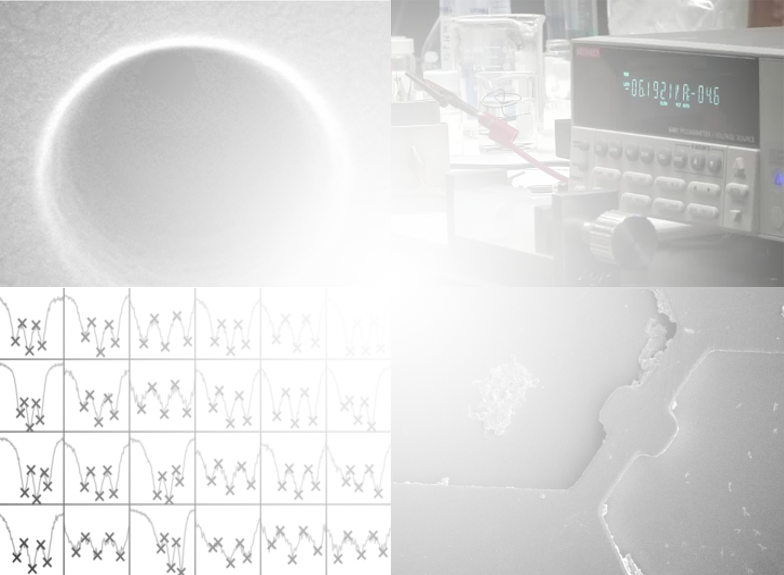
\includegraphics[width=\paperwidth,height=\paperheight]{title_image.png}}}
\begin{frame}[c]
 \begin{center}
  

  
  % Title
  \Huge{
	\textcolor{gray0}{Resistive-pulse sensing at the micro- and nanoscale}
  }
  
  
  % Name --- Institution
  \vspace{.25in}
  {\Large 
	\textcolor{gray1}{Preston Hinkle} \hspace{.5in} 
\includegraphics[height=1em]{uci_wordmark.png}
  }
  
  
  % Talk location
  \vspace{.5in}
  {\small
	\textit{\today}
  }
  
  
  
 \end{center}

\end{frame}
}



%%%%%%%%%%%%%%%%%%%%%%%%%%%%%%%%%%%%%%%%%%%%%%%%%%%%%%%%%%%%%%%%%%%%%%%%%%%%%%%%%%%%%%%%%%%%%%%%%%%%%%%%%%%%%%%%%%%%%%%%%%%%
% Outline
%%%%%%%%%%%%%%%%%%%%%%%%%%%%%%%%%%%%%%%%%%%%%%%%%%%%%%%%%%%%%%%%%%%%%%%%%%%%%%%%%%%%%%%%%%%%%%%%%%%%%%%%%%%%%%%%%%%%%%%%%%%%


\begin{frame}[c]{Outline}
 
	\begin{columns}[t]
		\begin{column}[T]{2.25in}
		
			\setbeamercovered{transparent}
			\begin{itemize}
				\item\only<1>{\textcolor{porestatsblack}{Resistive pulse sensing background}}\only<2,3,4>{\textcolor{ucigray0}{Resistive pulse sensing background}}
				\item\only<2>{\textcolor{porestatsblack}{Resistive pulse sensing of high-aspect ratio particles}}\only<1,3,4>{\textcolor{ucigray0}{Resistive pulse sensing of high-aspect ratio particles}}	
				\item\only<3,4>{\textcolor{porestatsblack}{Microscale resistive pulse sensing}}\only<1,2>{\textcolor{ucigray0}{Microscale resistive pulse sensing}}
				
					\begin{itemize}
						\item\only<3>{\textcolor{porestatsblack}{Simultaneous imaging and resistive pulse studies}}\only<1,2,4>{\textcolor{ucigray0}{Simultaneous imaging and resistive pulse studies}}
						\item\only<4>{\textcolor{porestatsblack}{Cancer cell deformability cytometry}}\only<1,2,3>{\textcolor{ucigray0}{Cancer cell deformability cytometry}}
					\end{itemize}
					
					
				
			\end{itemize}
			\setbeamercovered{invisible}
			
		\end{column}
		
		
		\begin{column}[T]{2.25in}
	
		
			% RP Background 1
			\onslide<1>{
				\begin{picture}(0,0)(0,0)
					\put(0,-180)
					{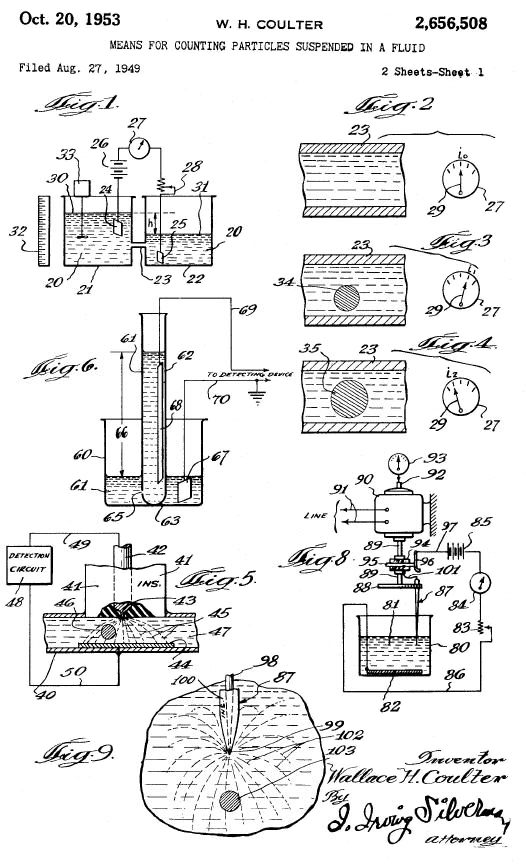
\includegraphics[width=2in]{coulter_patent_drawing}}
				\end{picture}
			}

		
			% Rods 1
			\onslide<2>{
				\begin{picture}(0,0)(0,0)
					\put(10,-30)
					{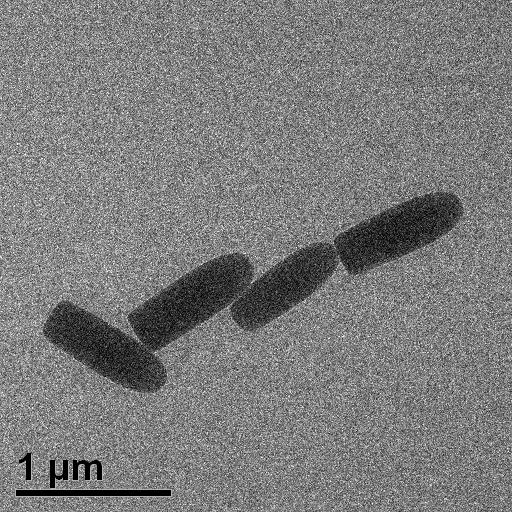
\includegraphics[width=1.25in]{shortrods}}
				\end{picture}
			}
			
			% Rods 2
			\onslide<2>{
				\begin{picture}(0,0)(0,0)
					\put(50,-125)
					{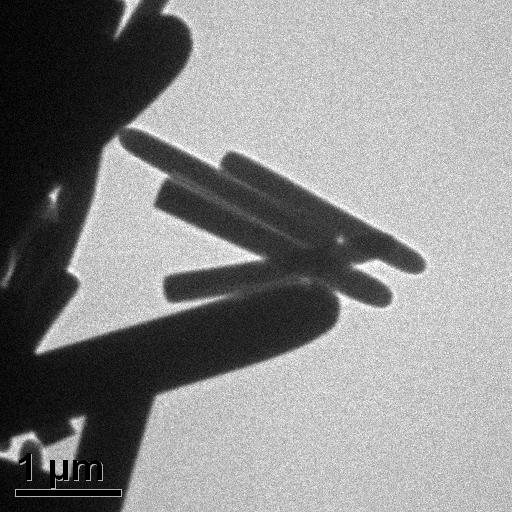
\includegraphics[width=1.25in]{longrods}}
				\end{picture}
			}
			
			
			% RPIM 1
			\onslide<3>{
				\begin{picture}(0,0)(0,0)
					\put(0, -65)
					{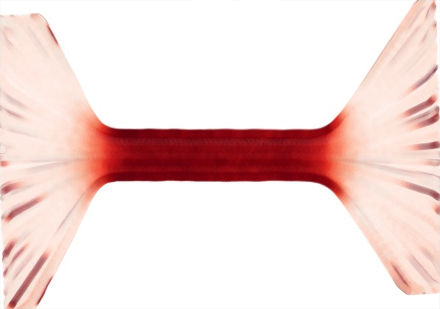
\includegraphics[width=2.25in]{resistancemap}}
				\end{picture}
			}
			
			% Cells
			\onslide<4>{
				\begin{picture}(0,0)(0,0)
					\put(0, -75)
					{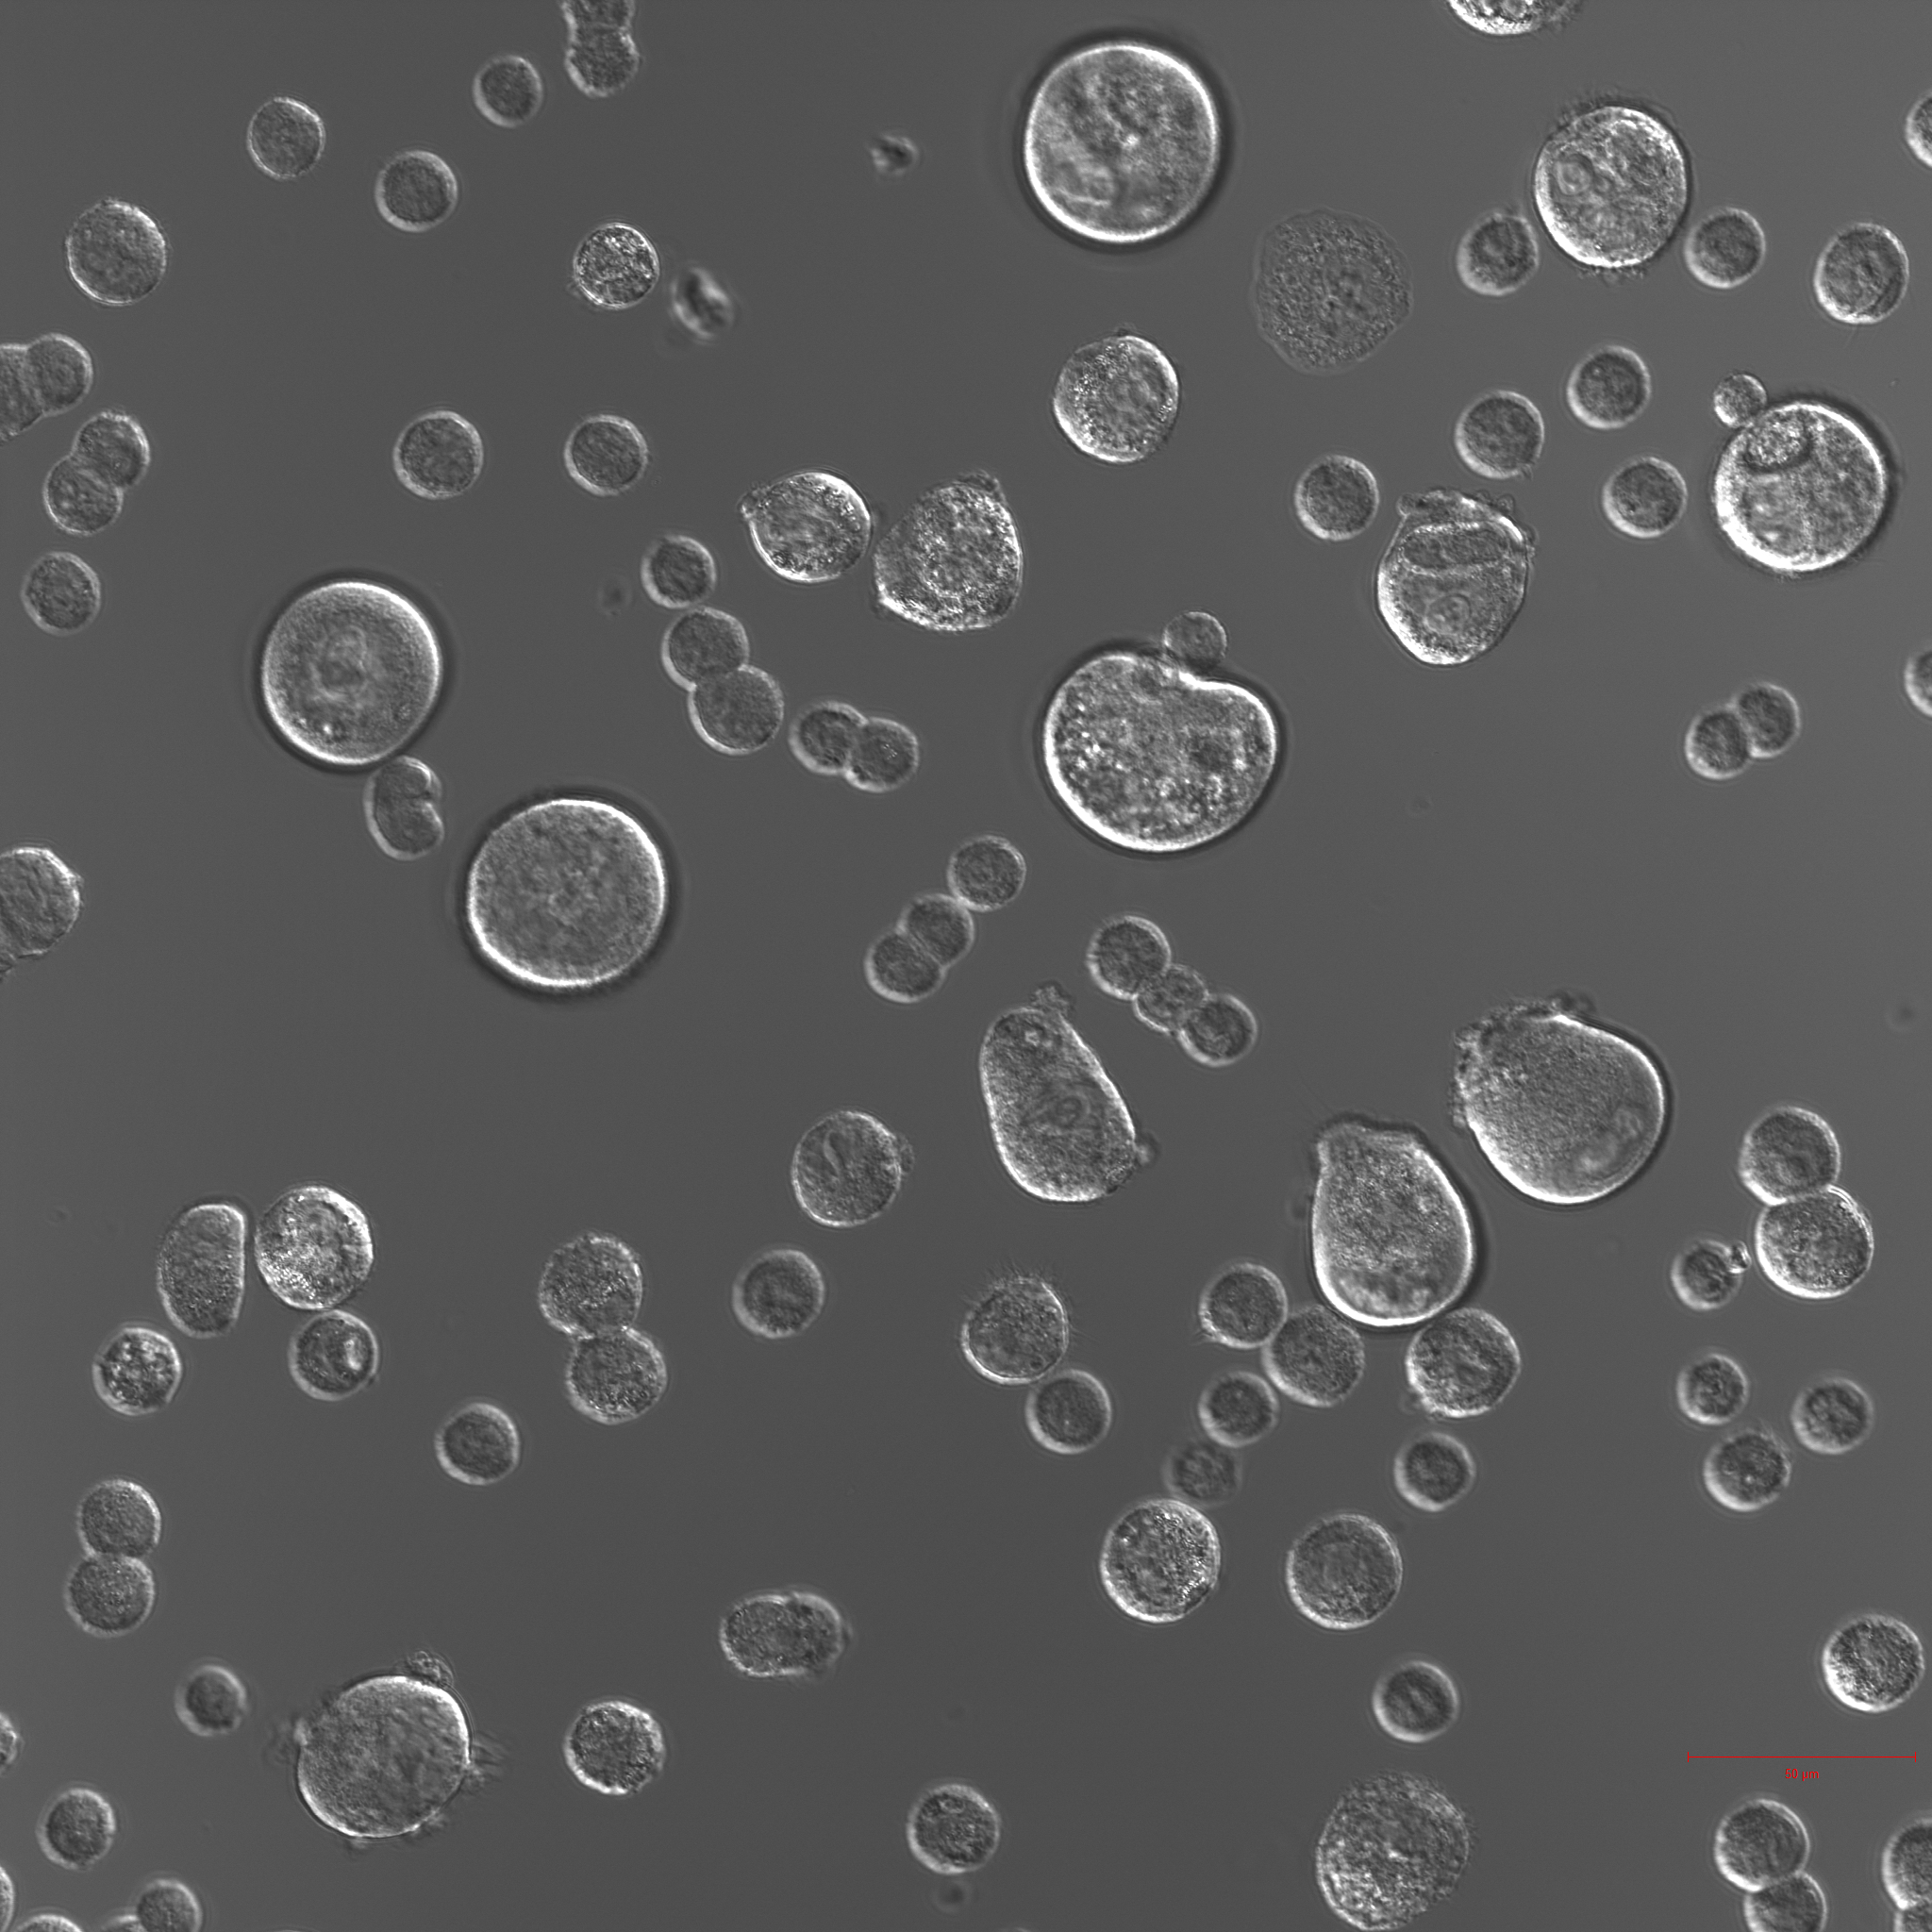
\includegraphics[width=2.25in]{cells}}
				\end{picture}
			}


			
			
		\end{column}
		
	\end{columns}

	
	
	
	
	
\end{frame}


%%%%%%%%%%%%%%%%%%%%%%%%%%%%%%%%%%%%%%%%%%%%%%%%%%%%%%%%%%%%%%%%%%%%%%%%%%%%%%%%%%%%%%%%%%%%%%%%%%%%%%%%%%%%%%%%%%%%%%%%%%%%
% Resistive pulse background title slide
%%%%%%%%%%%%%%%%%%%%%%%%%%%%%%%%%%%%%%%%%%%%%%%%%%%%%%%%%%%%%%%%%%%%%%%%%%%%%%%%%%%%%%%%%%%%%%%%%%%%%%%%%%%%%%%%%%%%%%%%%%%%


\begin{frame}[c]{}
	\begin{center}
		\textbf{Resistive pulse sensing background}
	\end{center}
\end{frame}



%%%%%%%%%%%%%%%%%%%%%%%%%%%%%%%%%%%%%%%%%%%%%%%%%%%%%%%%%%%%%%%%%%%%%%%%%%%%%%%%%%%%%%%%%%%%%%%%%%%%%%%%%%%%%%%%%%%%%%%%%%%%
% Resistive pulse background---description
%%%%%%%%%%%%%%%%%%%%%%%%%%%%%%%%%%%%%%%%%%%%%%%%%%%%%%%%%%%%%%%%%%%%%%%%%%%%%%%%%%%%%%%%%%%%%%%%%%%%%%%%%%%%%%%%%%%%%%%%%%%%


\begin{frame}[c]{Resistive pulse sensing---description}
	
	\begin{columns}[t]
		\begin{column}[T]{2.75in}
	
			\begin{itemize}
				\item Resistive pulse sensing (RP) is a method for single particle detection and characterization
				\item Works at any scale (nano, micro, milli, etc.)
				\item A diverse range of applications: red blood cell counting (several $\SI{}{\mu m}$, virus detection ($10-\SI{100}{\mu m}$, and DNA sequencing ($\sim\SI{1}{nm}$), among others
			\end{itemize}
	
		\end{column}
		
		\begin{column}[T]{1.75in}
			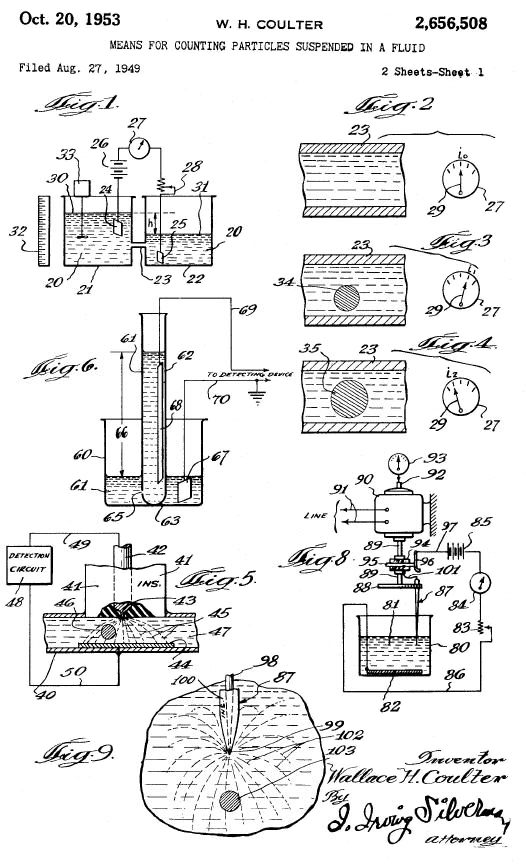
\includegraphics[width=1.75in]{coulter_patent_drawing.png}
		\end{column}
		
	\end{columns}

	
\end{frame}



%%%%%%%%%%%%%%%%%%%%%%%%%%%%%%%%%%%%%%%%%%%%%%%%%%%%%%%%%%%%%%%%%%%%%%%%%%%%%%%%%%%%%%%%%%%%%%%%%%%%%%%%%%%%%%%%%%%%%%%%%%%%
% Resistive pulse background---how does it work?
%%%%%%%%%%%%%%%%%%%%%%%%%%%%%%%%%%%%%%%%%%%%%%%%%%%%%%%%%%%%%%%%%%%%%%%%%%%%%%%%%%%%%%%%%%%%%%%%%%%%%%%%%%%%%%%%%%%%%%%%%%%%


\begin{frame}[c]{Resistive pulse sensing---how does it work?}

	\begin{columns}[t]
		\begin{column}[T]{2.75in}
	      
	

			\begin{tiny}
				\begin{itemize}
				
					\item A nanopore immersed in electrolyte solution acts as an ionic resistor
					\item Current-Voltage relationship follows Ohm's law $V=IR$
					\item When a particle enters the channel its resistance changes, yielding a pulse in the measured ionic current
					\item Pulse properties yield information on size, shape, charge, and concentration of particle
				\end{itemize}
				{\centering
					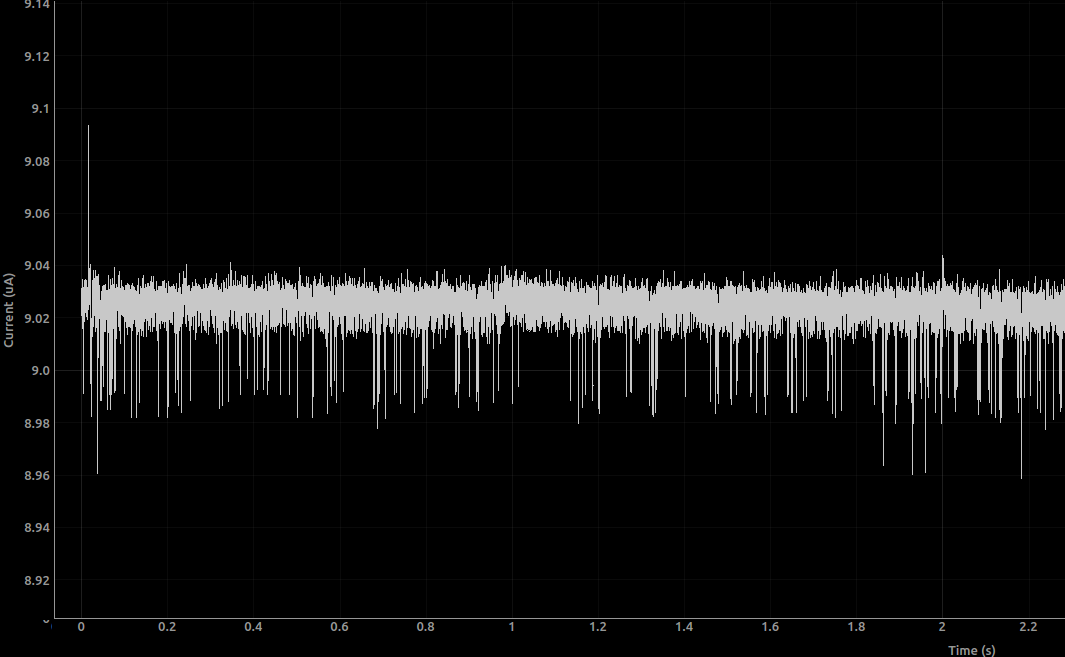
\includegraphics[height=1in,width=2.5in]{rp_timeseries.png} \\ \par
				}
			\end{tiny}
			
		\end{column}
		
		\begin{column}[T]{1.75in}
			{\centering
				\vspace{.5cm}
				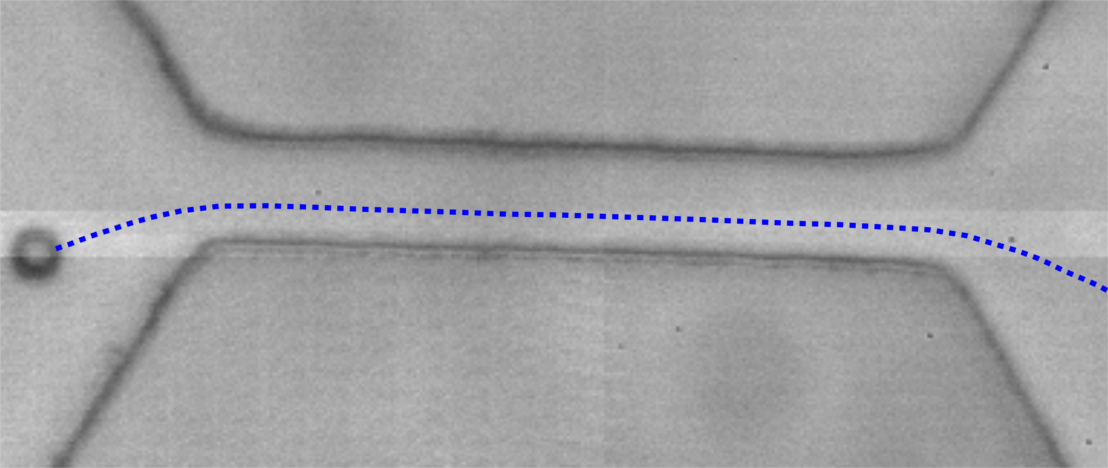
\includegraphics[width=1.5in]{singletrajectory} \\
				\vspace{.75cm}
				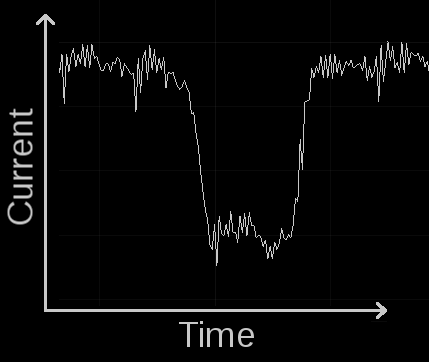
\includegraphics[width=1.5in]{singlerp} \\
				\par
			}
			
		\end{column}

	
	
	\end{columns}
	
\end{frame}




%%%%%%%%%%%%%%%%%%%%%%%%%%%%%%%%%%%%%%%%%%%%%%%%%%%%%%%%%%%%%%%%%%%%%%%%%%%%%%%%%%%%%%%%%%%%%%%%%%%%%%%%%%%%%%%%%%%%%%%%%%%%
% Resistive pulse background---system components
%%%%%%%%%%%%%%%%%%%%%%%%%%%%%%%%%%%%%%%%%%%%%%%%%%%%%%%%%%%%%%%%%%%%%%%%%%%%%%%%%%%%%%%%%%%%%%%%%%%%%%%%%%%%%%%%%%%%%%%%%%%%


\begin{frame}[c]{Resistive pulse sensing---system components}
	%\begin{picture}(0,0)(0,0)
		%\put(90,-125){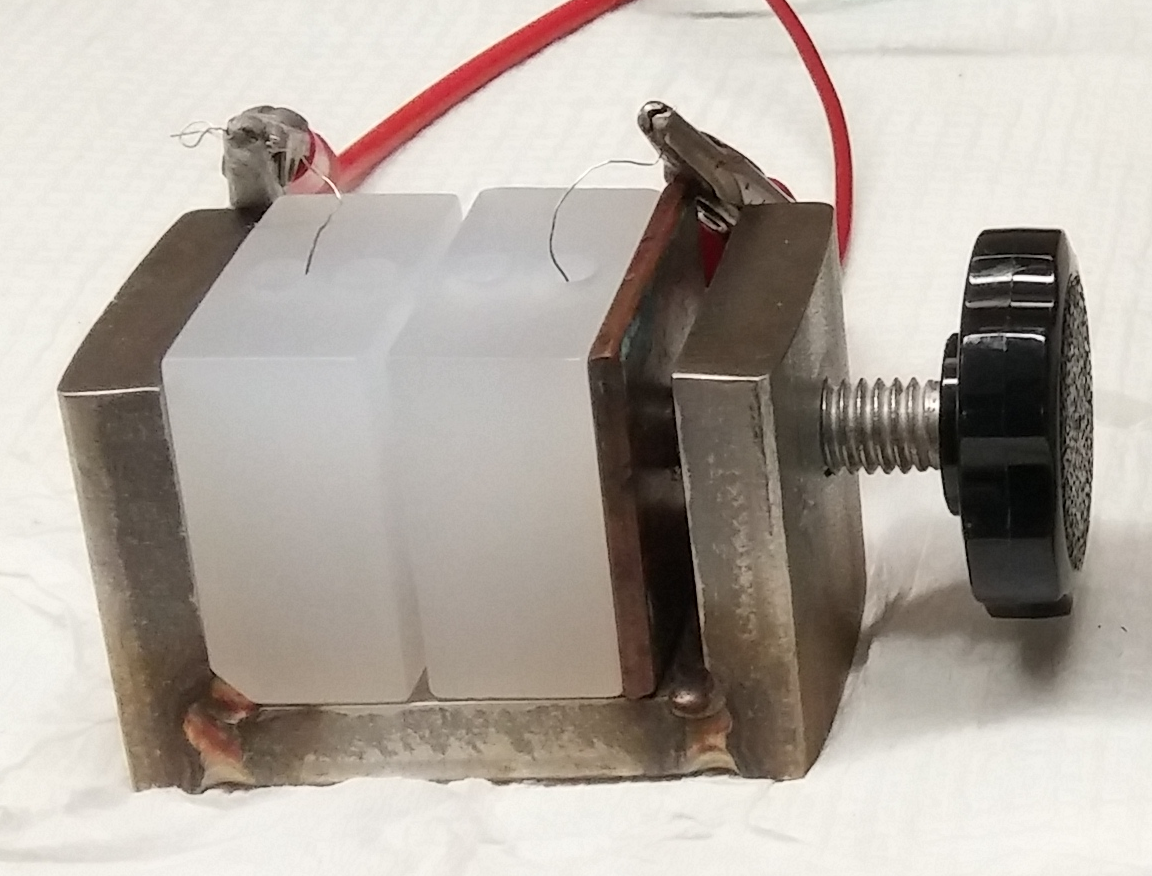
\includegraphics[width=7cm]{photo/conductivitycell.png}}
		%\put(100,0){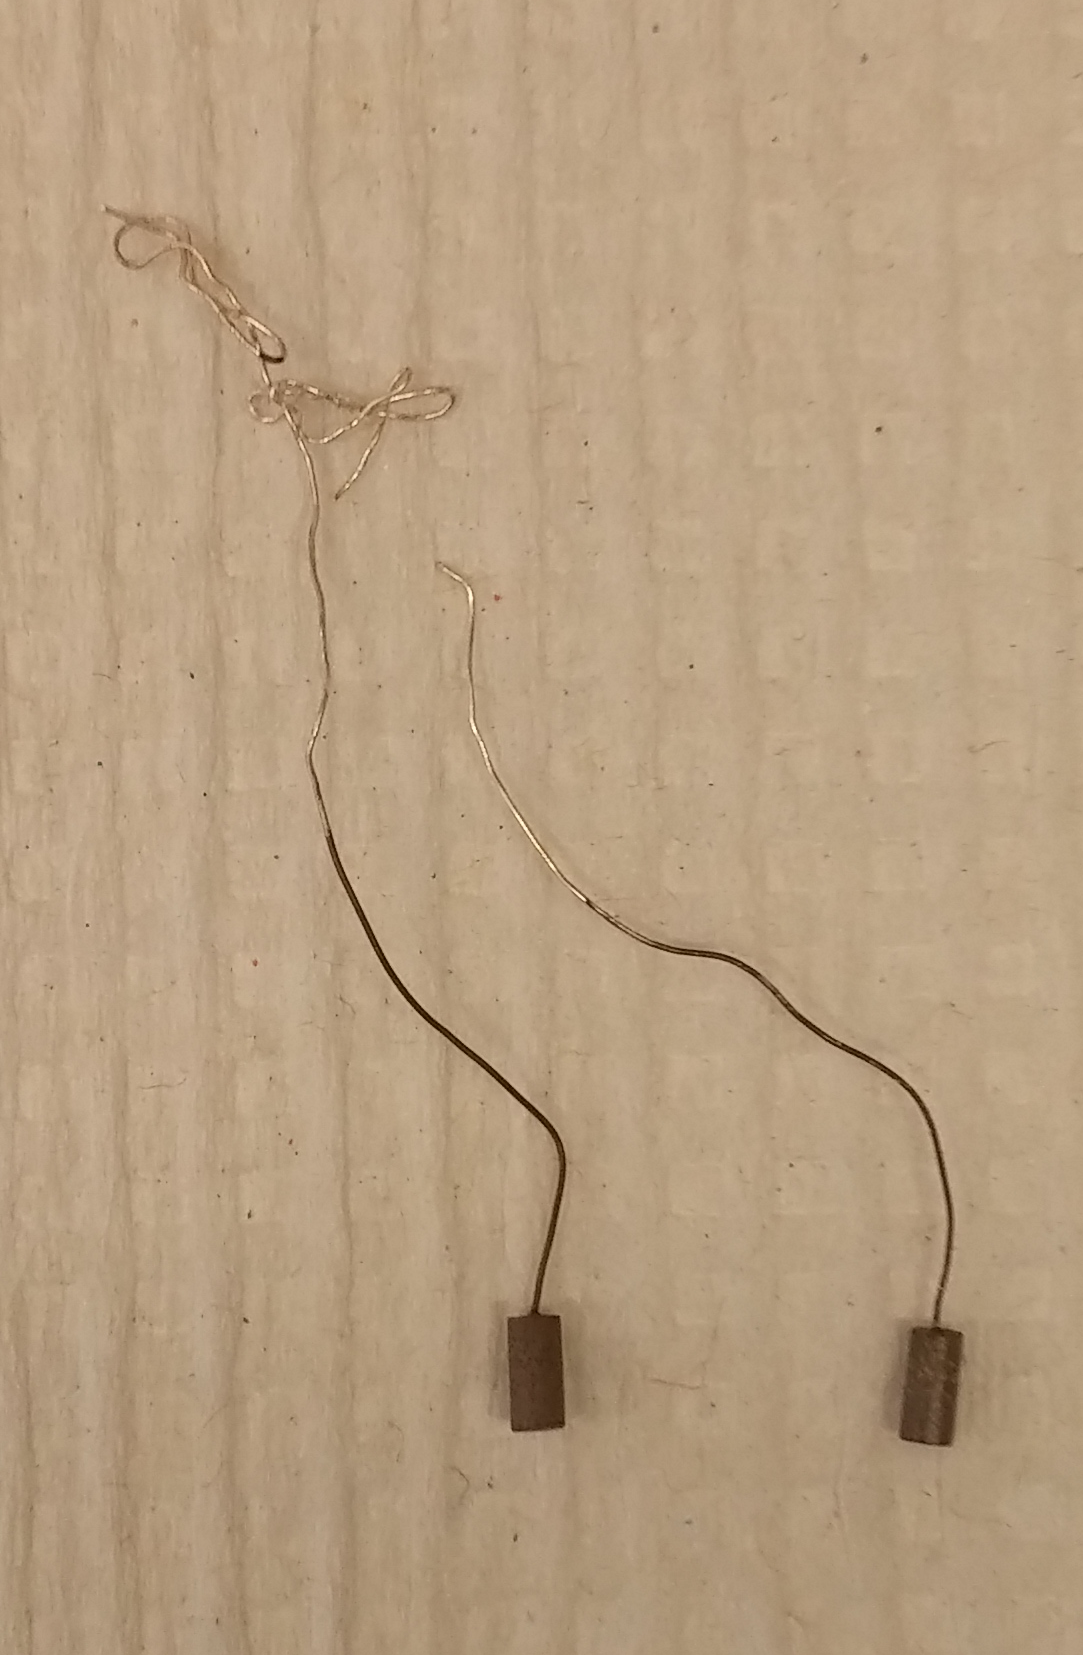
\includegraphics[width=2cm]{photo/electrodes.png}}
		%\put(10,-20){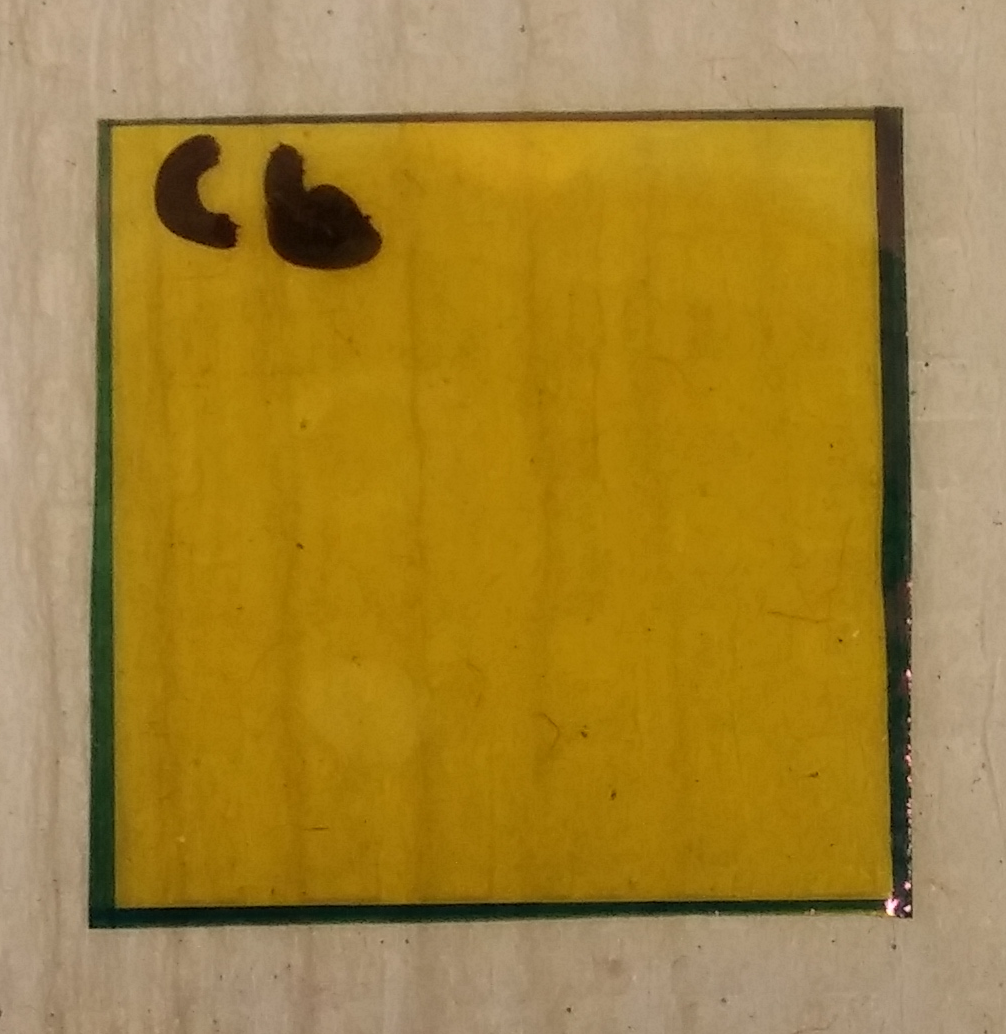
\includegraphics[width=2cm]{photo/membrane.png}}
		%\put(30,-80){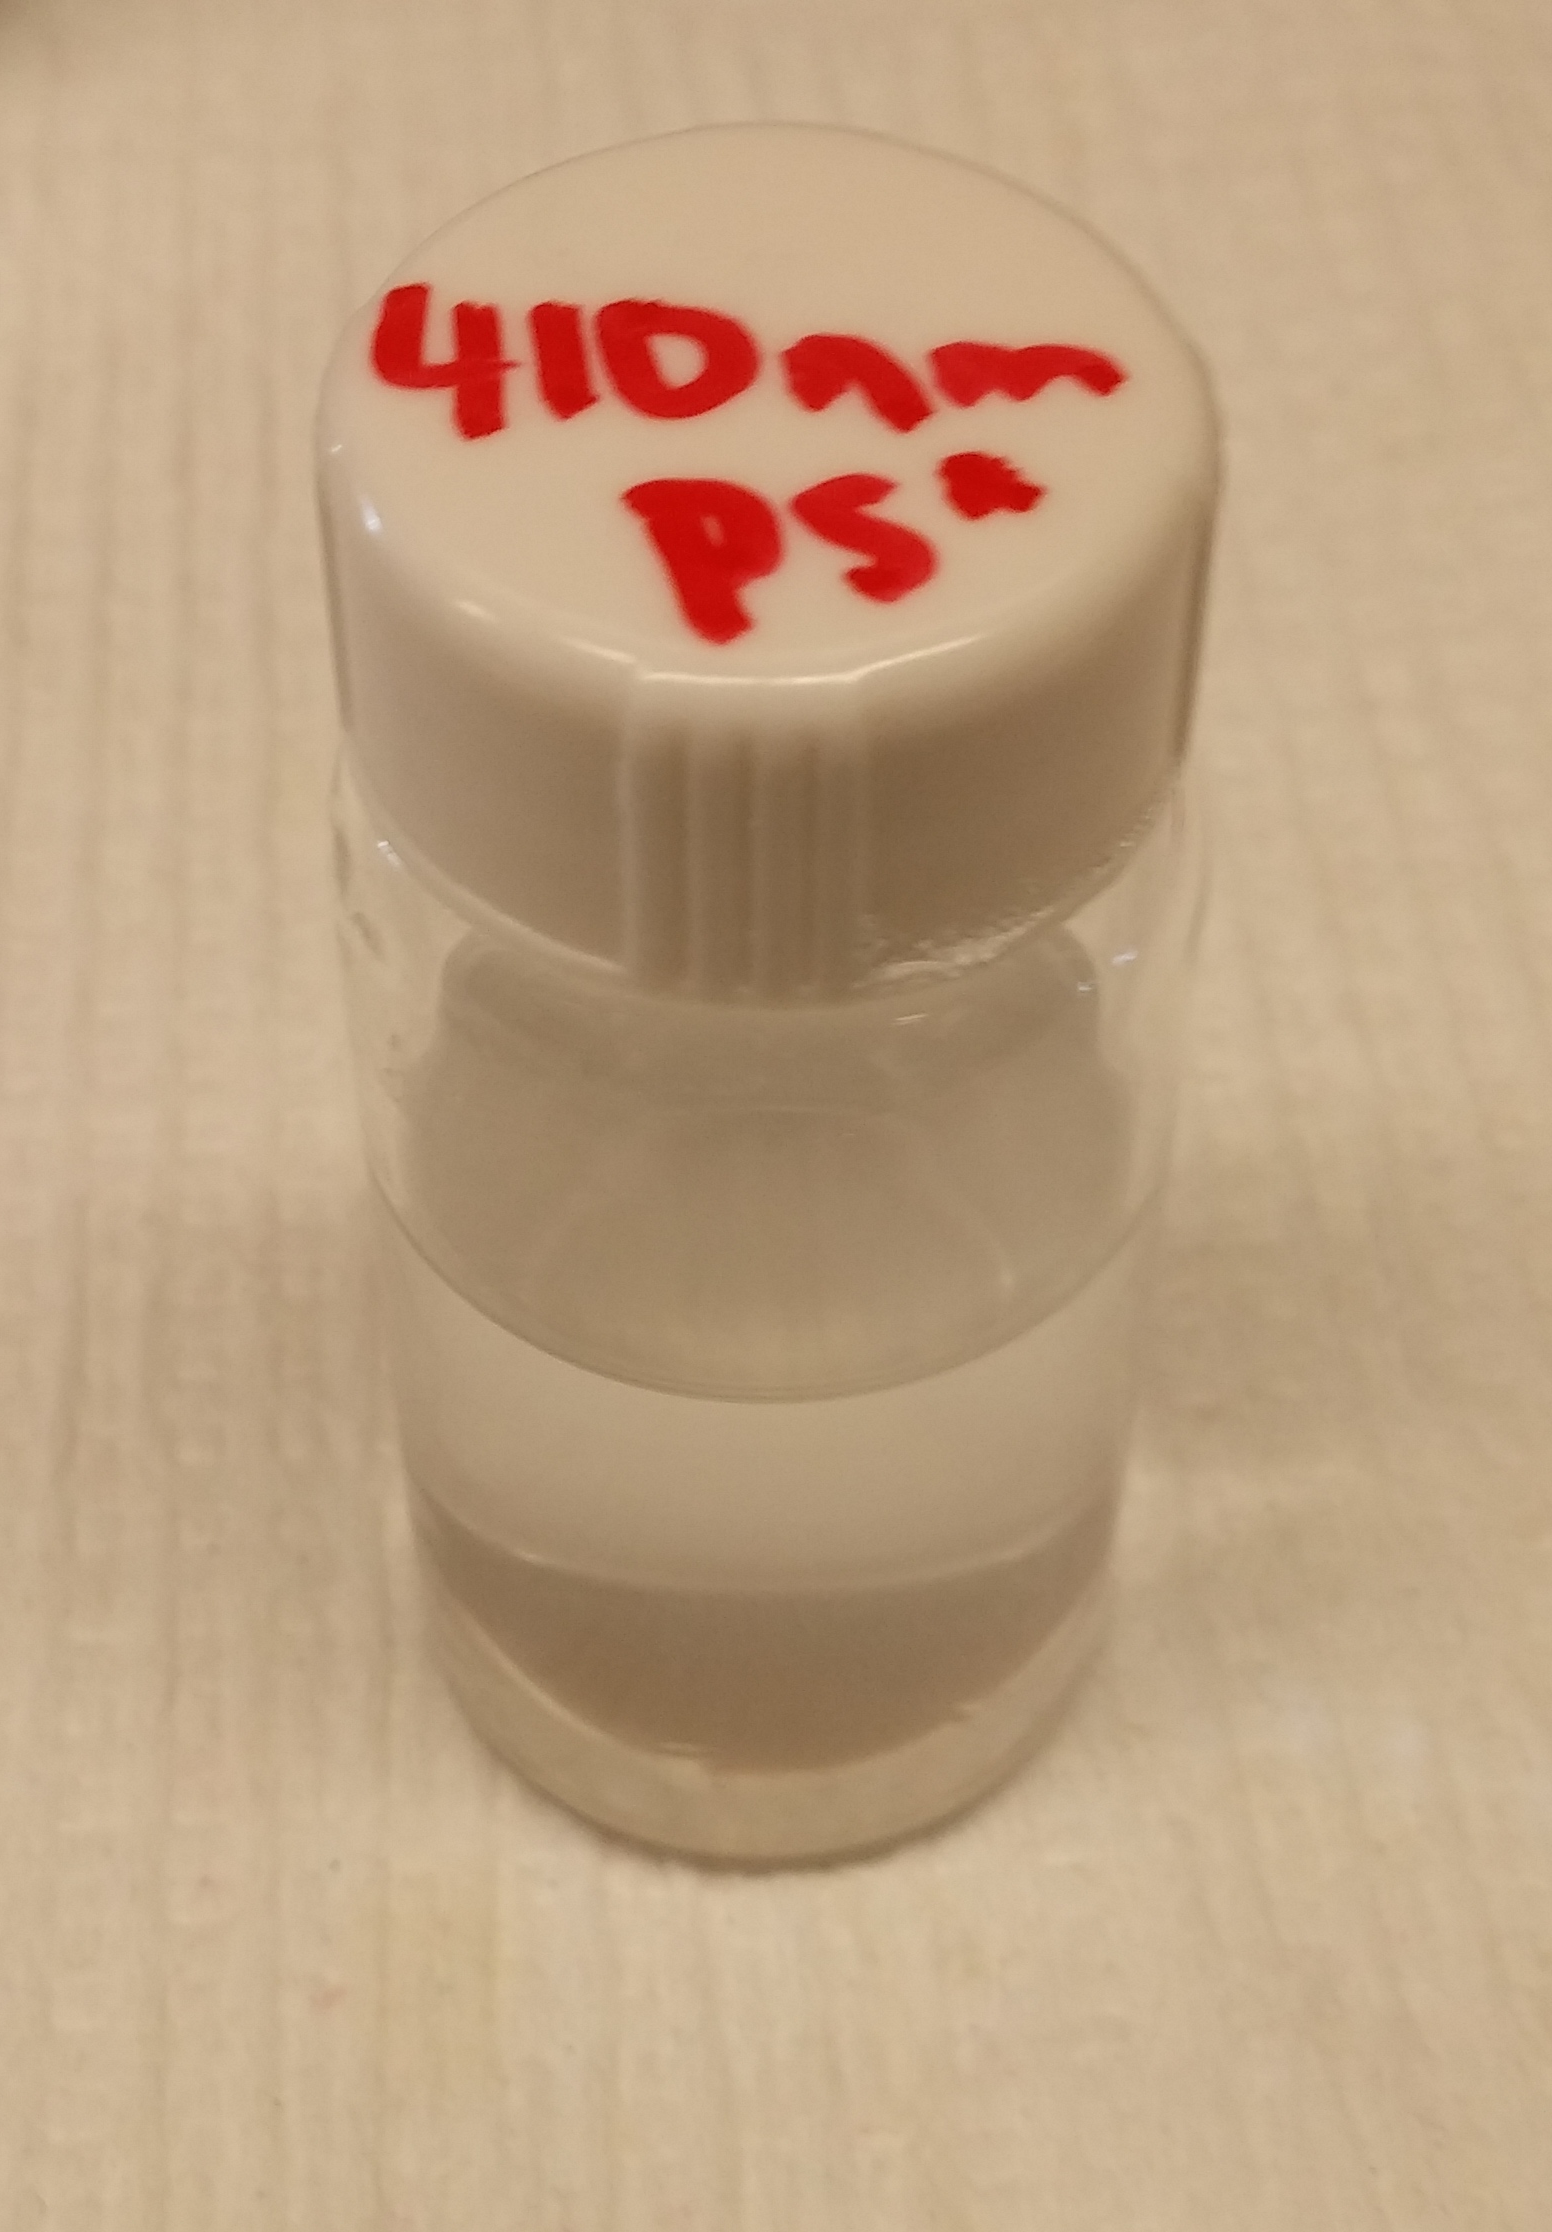
\includegraphics[width=2cm]{photo/solution.png}}
	%\end{picture}
% 	{\centering 
% 		\vspace{0.35cm}
% 		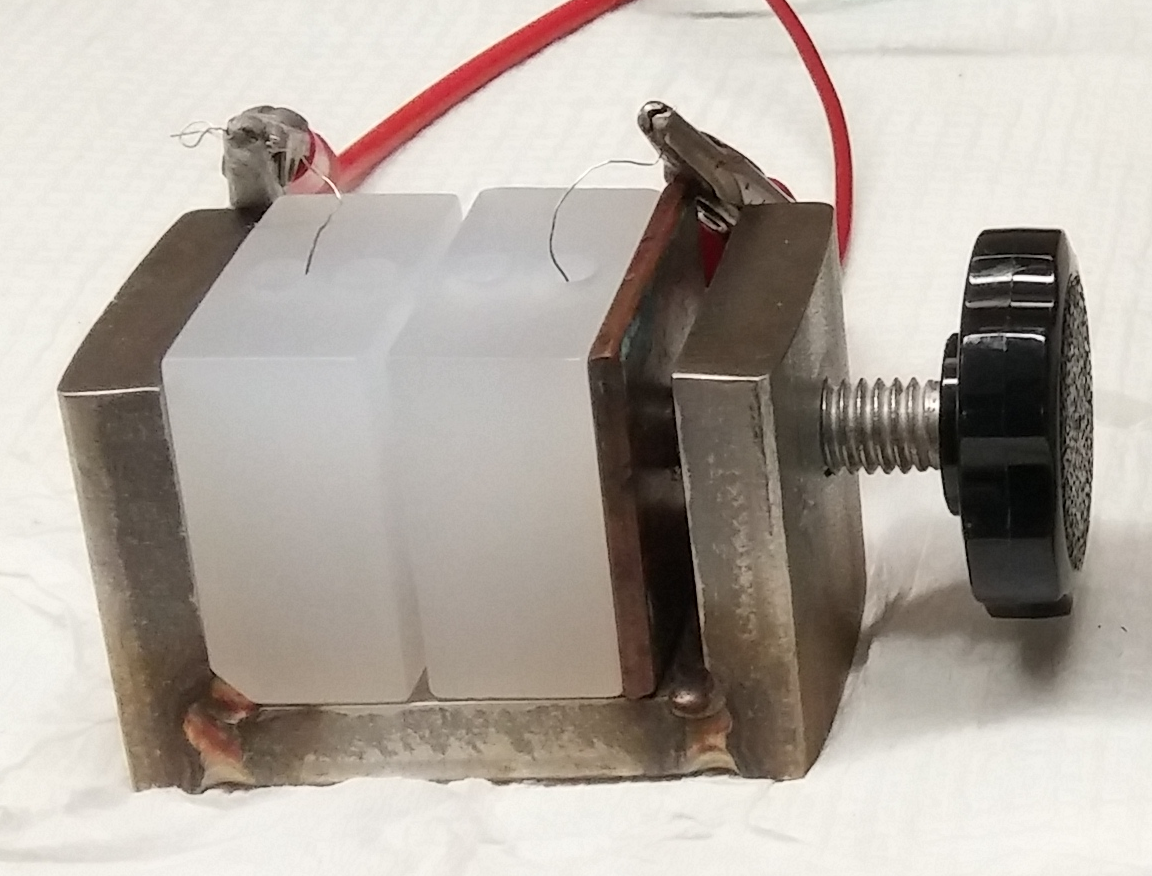
\includegraphics[width=9cm]{photo/conductivitycell.png}
% 		\newline
% 		\vspace{.35cm}
% 		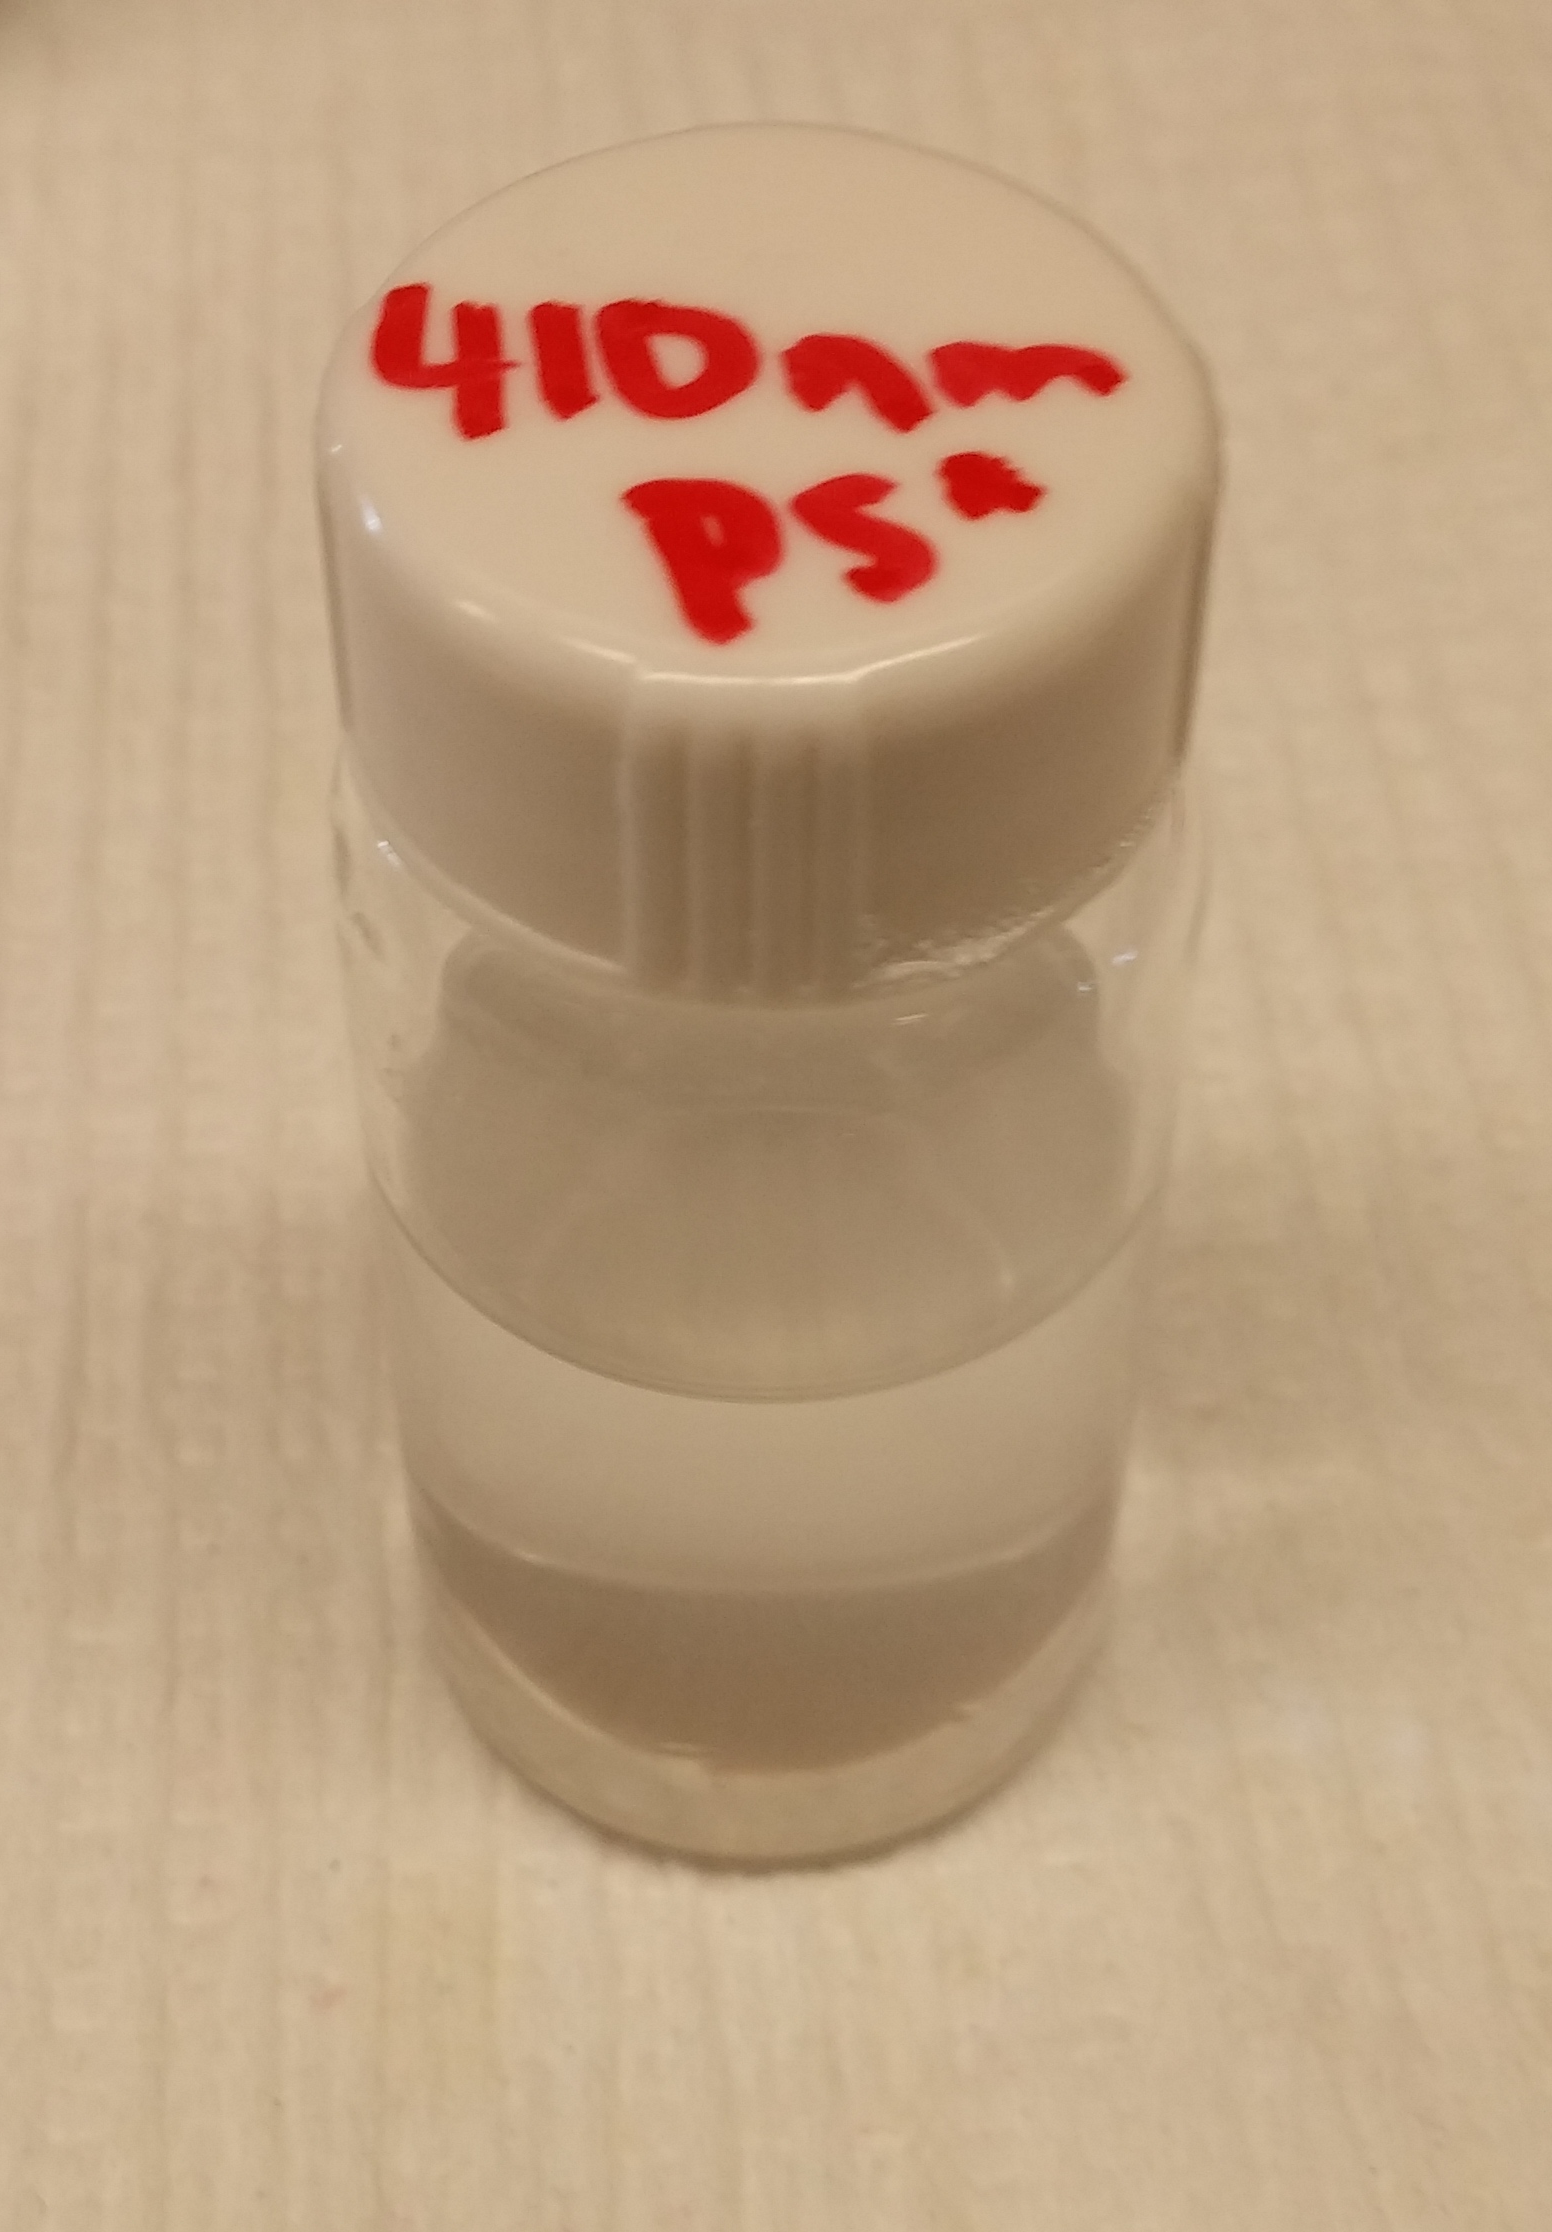
\includegraphics[width=1.5cm]{photo/solution.png}
% 		\hspace{1cm}
% 		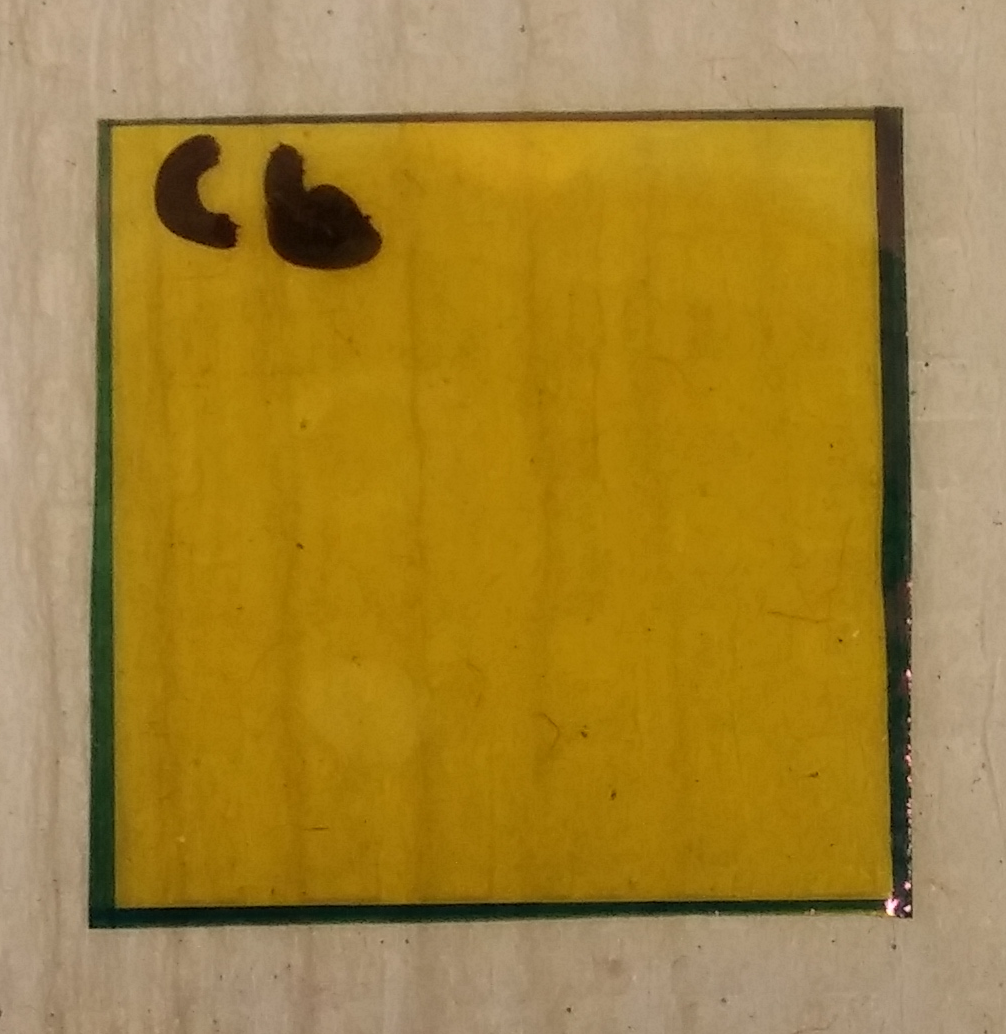
\includegraphics[width=2cm]{photo/membrane.png}
% 		\hspace{1cm}
% 		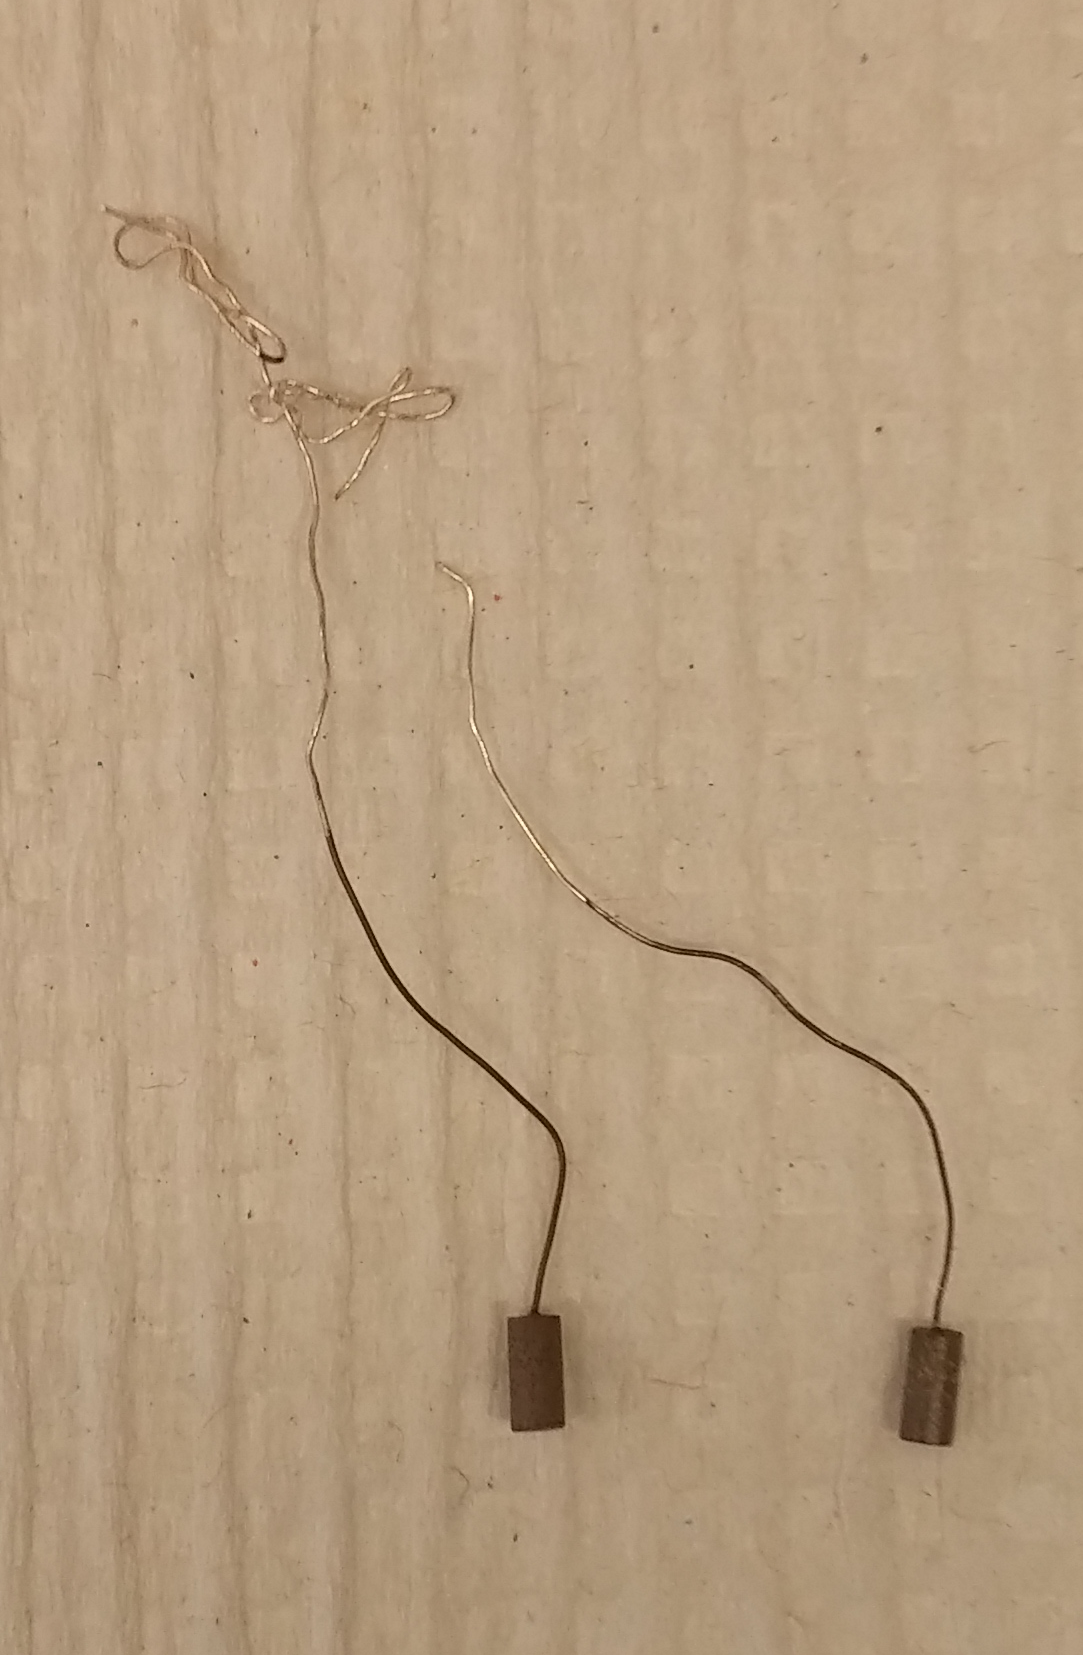
\includegraphics[width=1.5cm]{photo/electrodes.png}
% 		\hspace{1cm}
% 		\par
% 	}


	\begin{columns}[t]
		\begin{column}[T]{\paperwidth/5}
			{\centering
				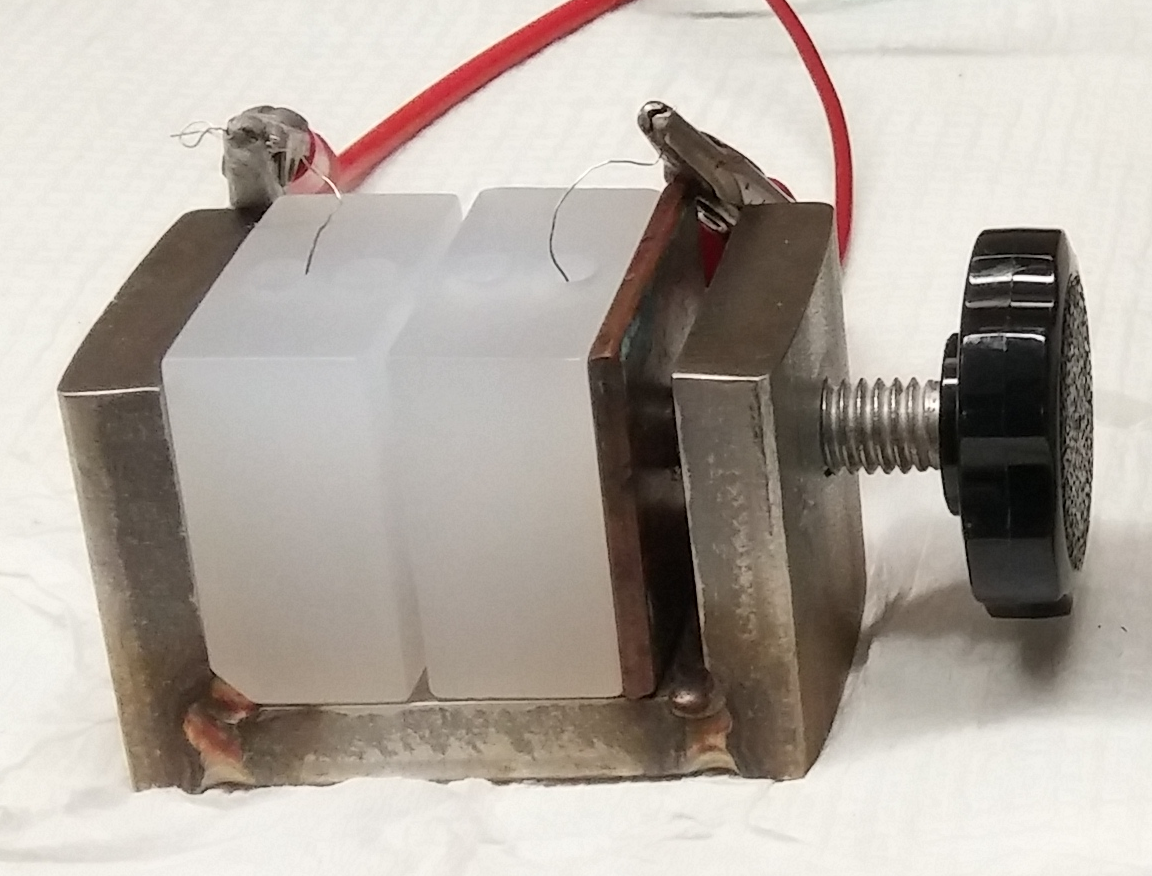
\includegraphics[height=2.25cm]{photo/conductivitycell.png} \\
				{\footnotesize Conductivity cell}
				\par
			}
		\end{column}
		
		
		\begin{column}[T]{\paperwidth/5}
			{\centering
				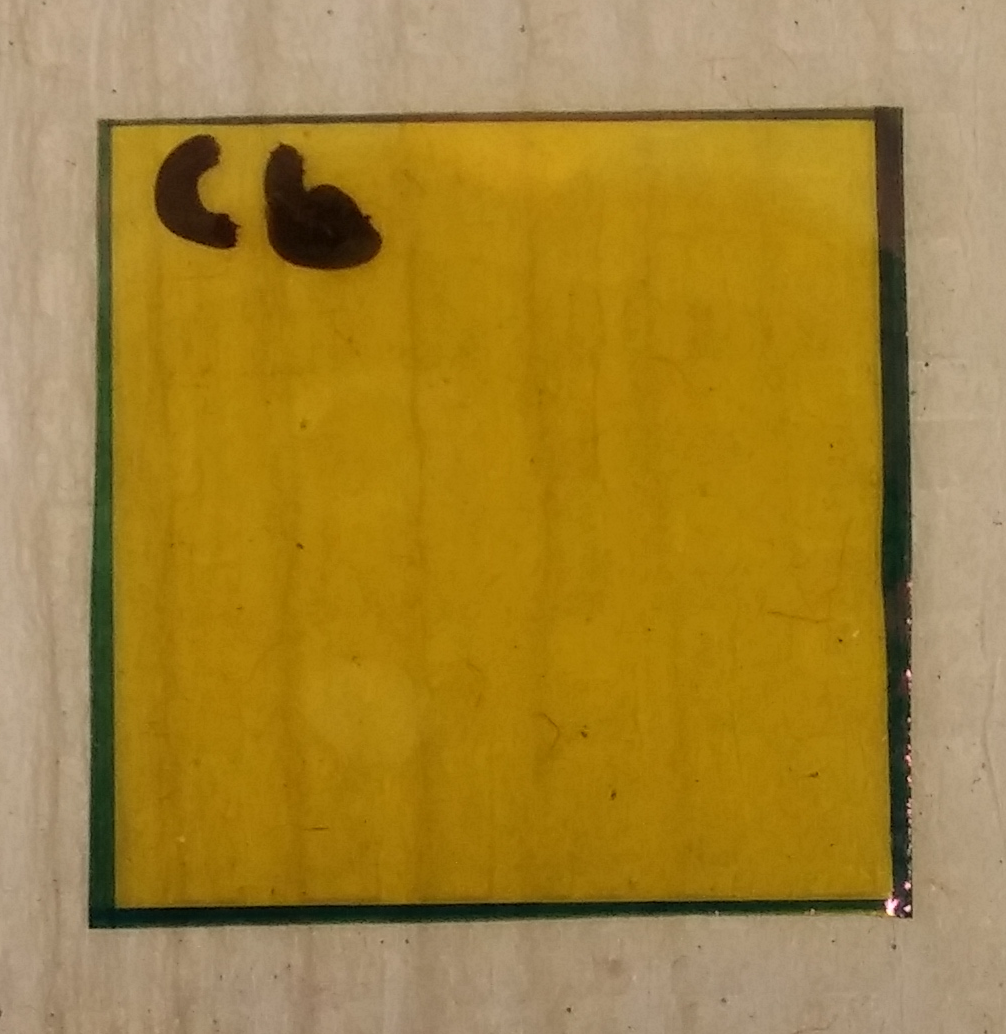
\includegraphics[height=2.25cm]{photo/membrane.png} \\
				{\footnotesize Pore membrane}
				\par
			}
		\end{column}
		
		
		
		\begin{column}[T]{\paperwidth/5}
			{\centering
				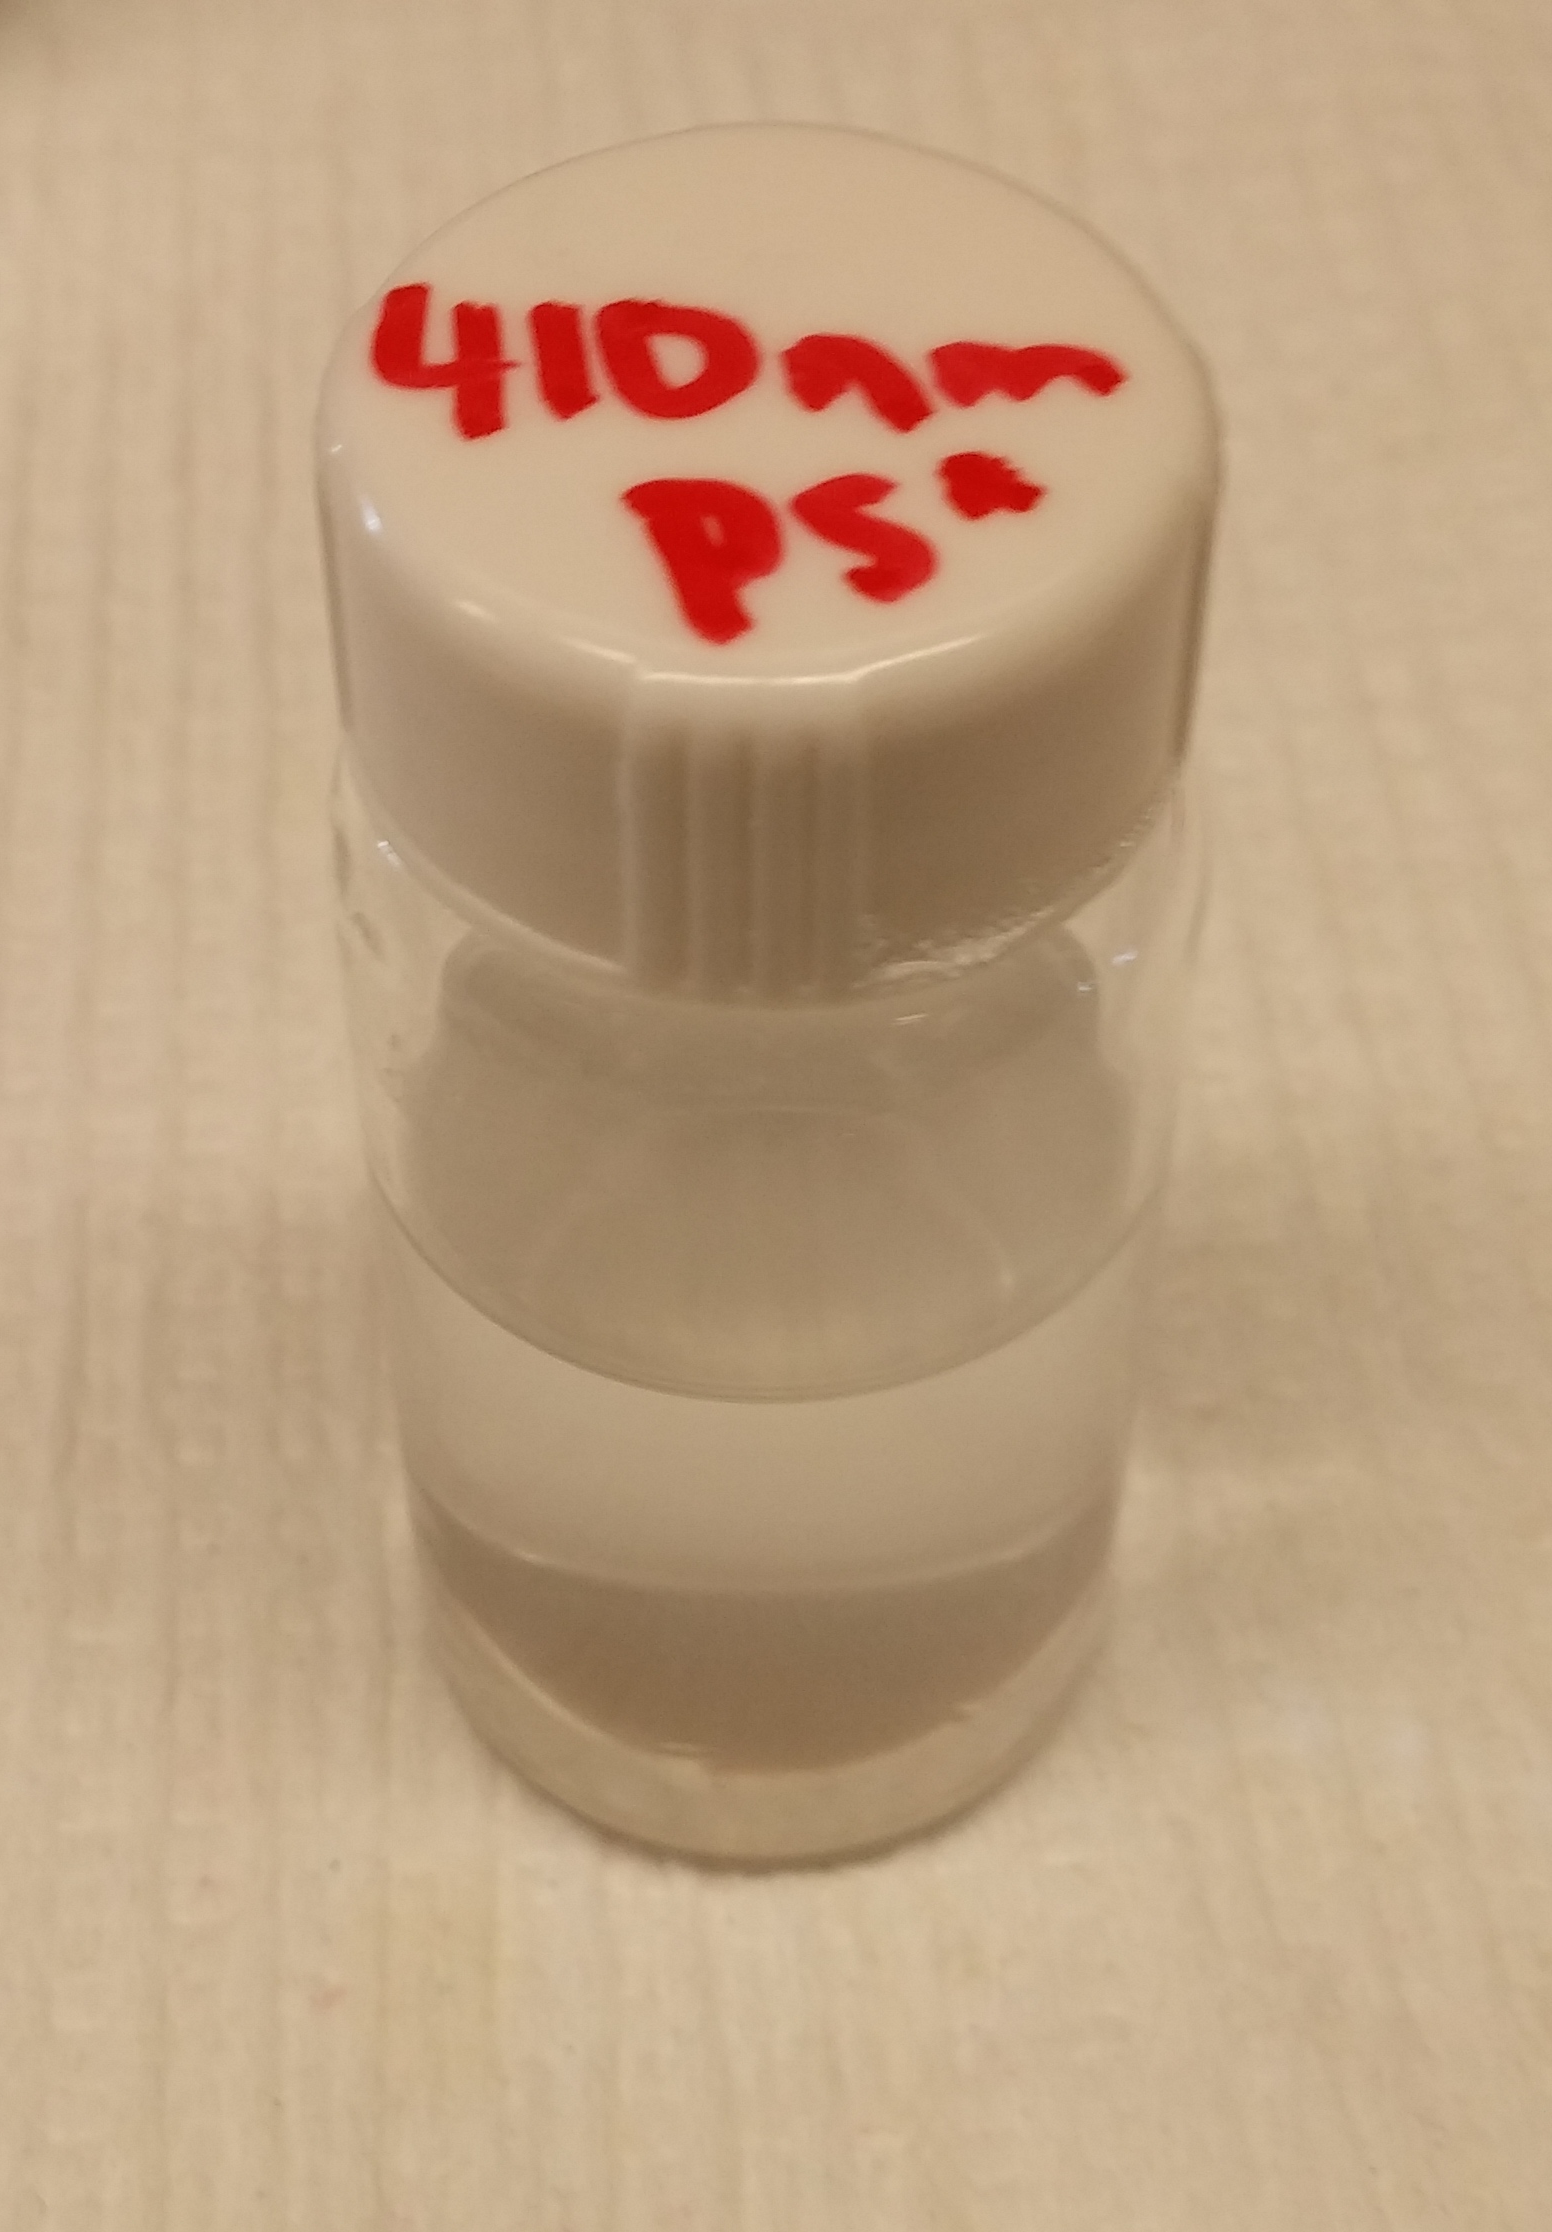
\includegraphics[height=2.25cm]{photo/solution.png} \\
				{\footnotesize Electrolyte}
				\par
			}
		\end{column}

		
		

		
		\begin{column}[T]{\paperwidth/5}
			{\centering
				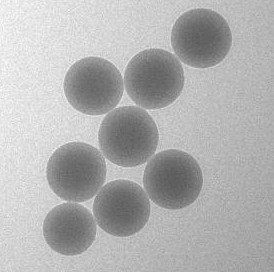
\includegraphics[height=2.25cm]{psbeads} \\
				{\footnotesize Particles}
				\par
			}
		\end{column}

	\end{columns}
	
	\vspace{1cm}
	
	\begin{columns}[t]
		\begin{column}[T]{\paperwidth/5}
			{\centering
				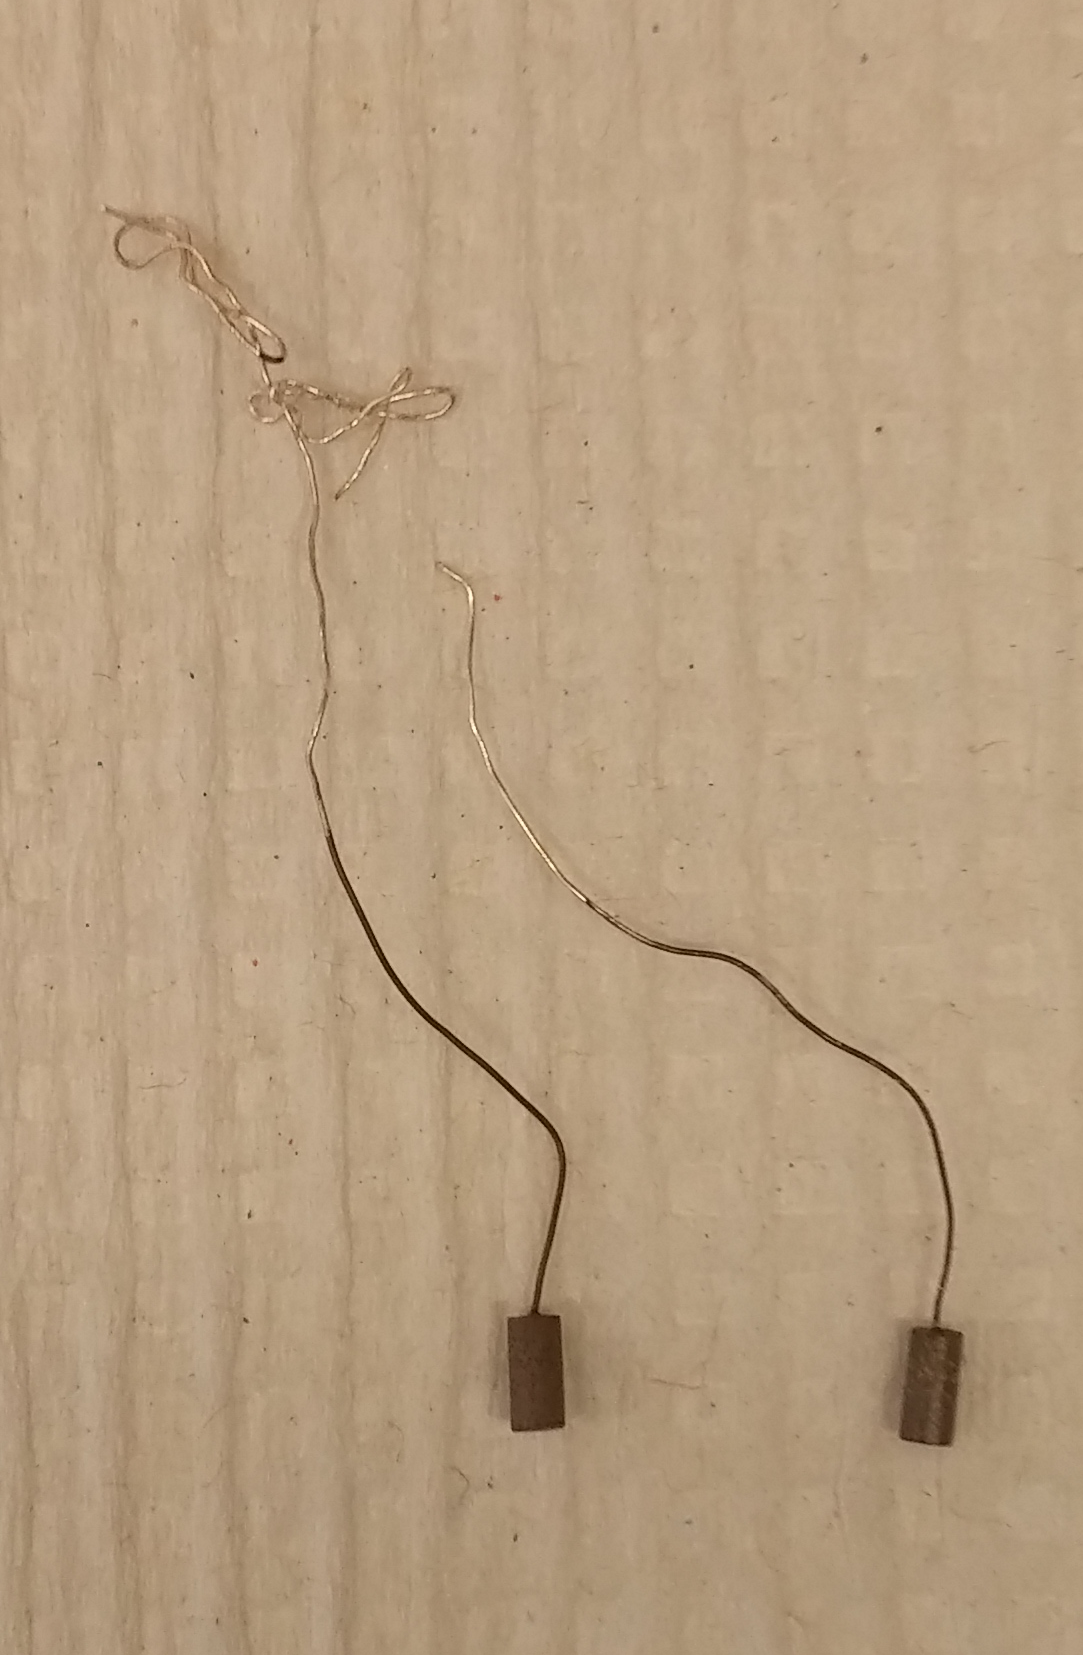
\includegraphics[height=2.25cm]{photo/electrodes.png} \\
				{\footnotesize Ag-AgCl electrodes}
				\par
			}
		\end{column}
		
		
		\begin{column}[T]{.6\paperwidth}
			{\centering
				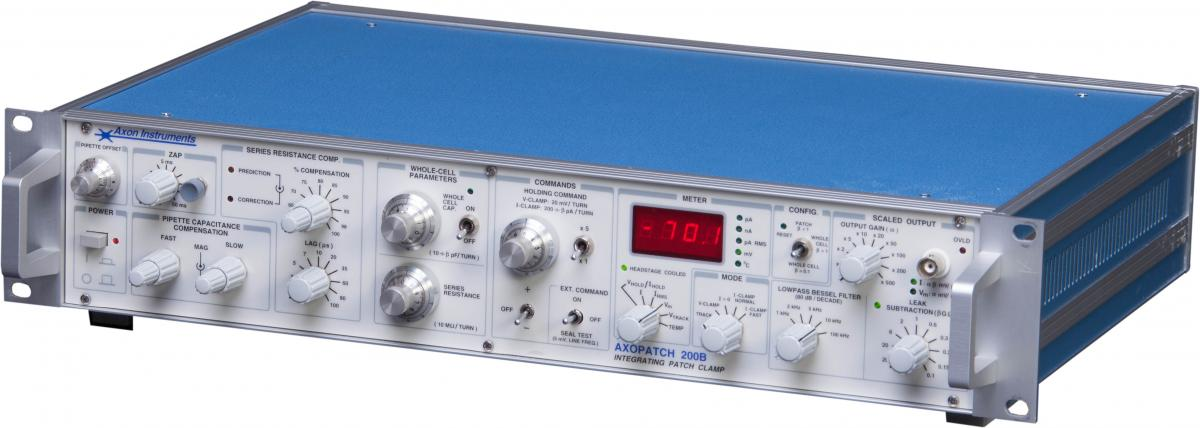
\includegraphics[height=2.25cm]{photo/axon200b} \\
				Voltage amplifier + current recorder
				\par
			}
		\end{column}
	

	\end{columns}




% 	
% 
% 
% 	\begin{center}
% 		\begin{figure}
% 		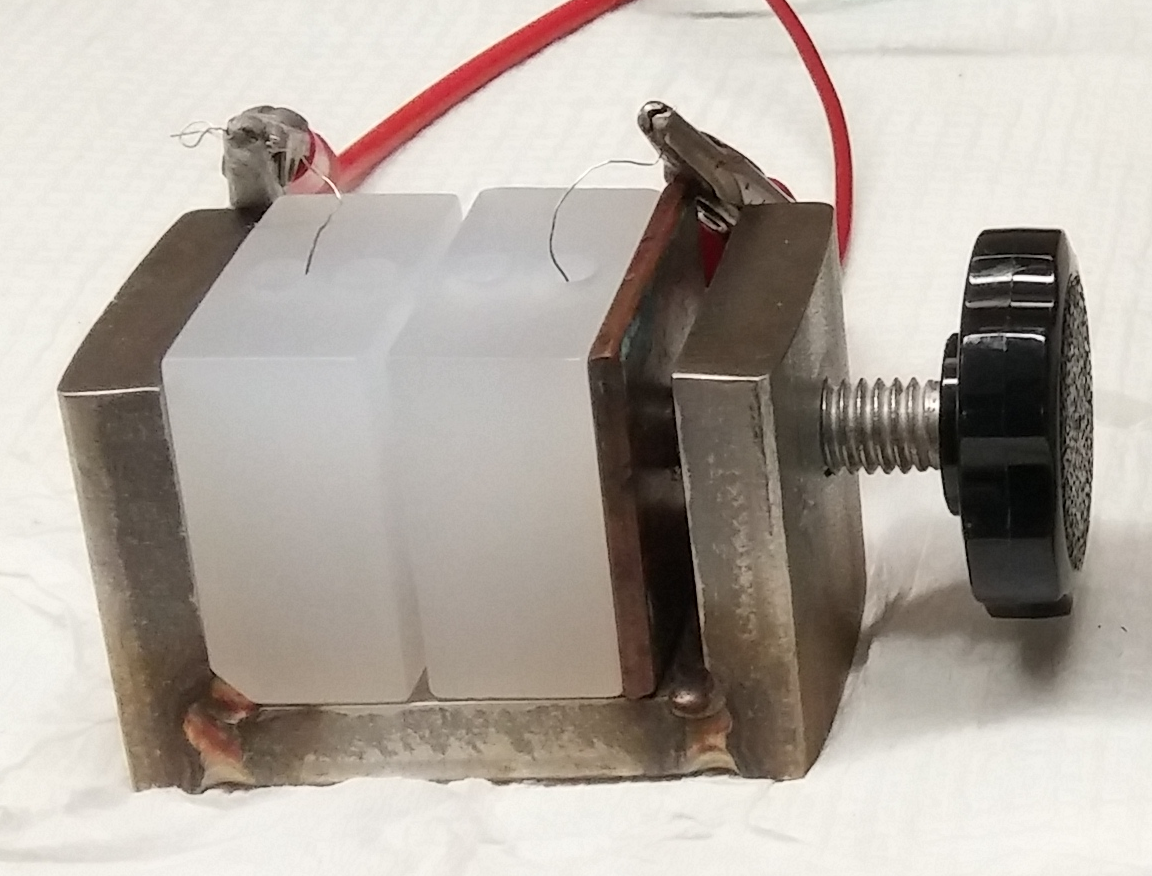
\includegraphics[height=2.25cm]{photo/conductivitycell.png}
% 		\caption{asdf}
% 		\end{figure}
% 		\hspace{.35cm}
%  		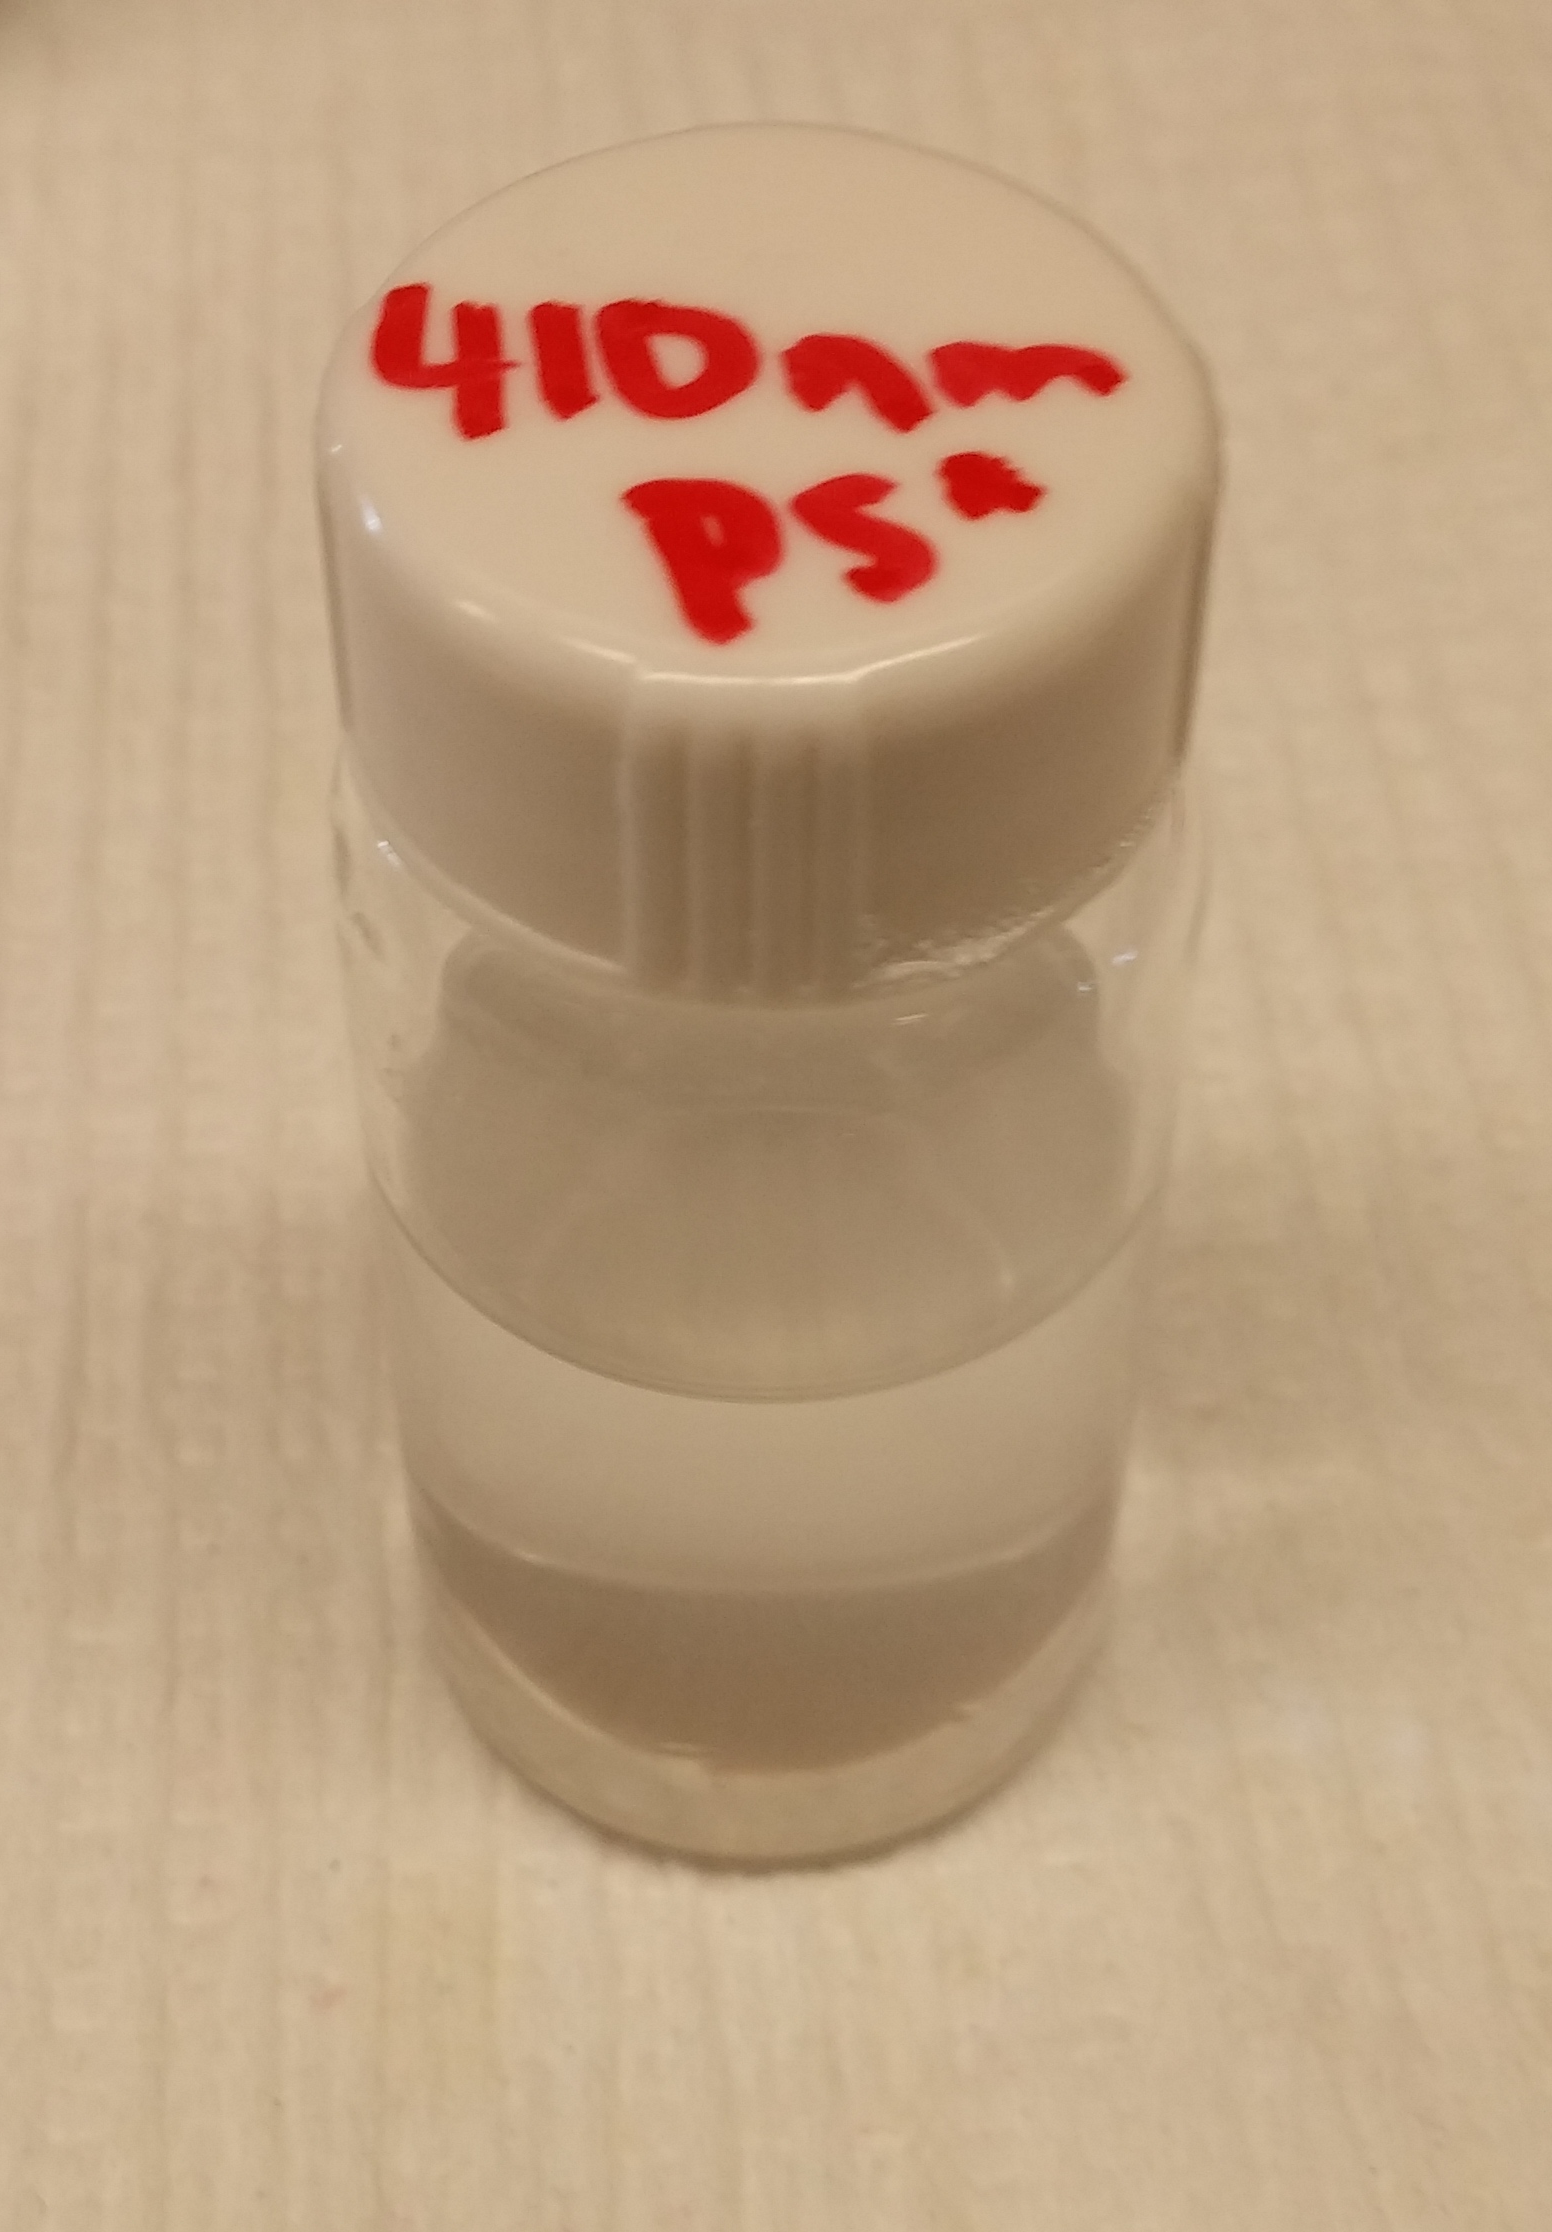
\includegraphics[height=2.25cm]{photo/solution.png}
%  		\hspace{.35cm}
%  		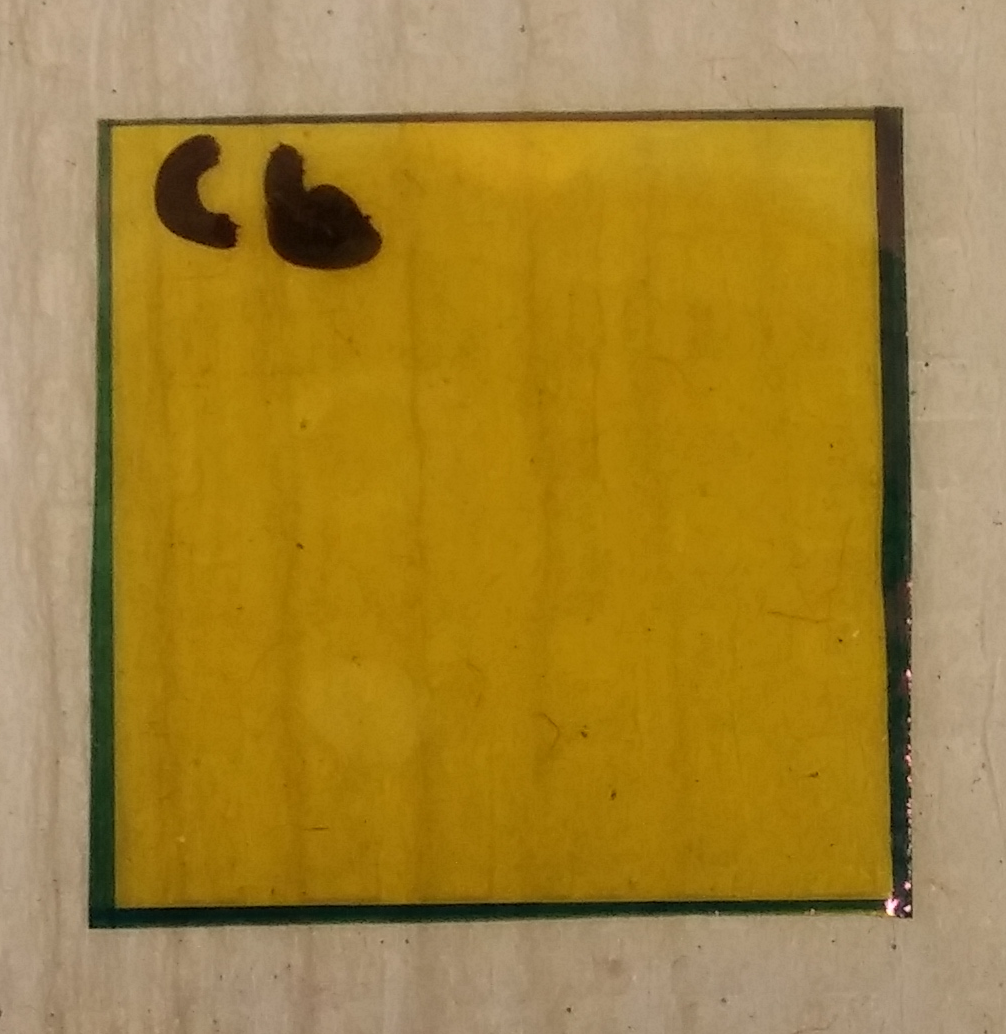
\includegraphics[height=2.25cm]{photo/membrane.png}
%  		\hspace{.35cm}
%  		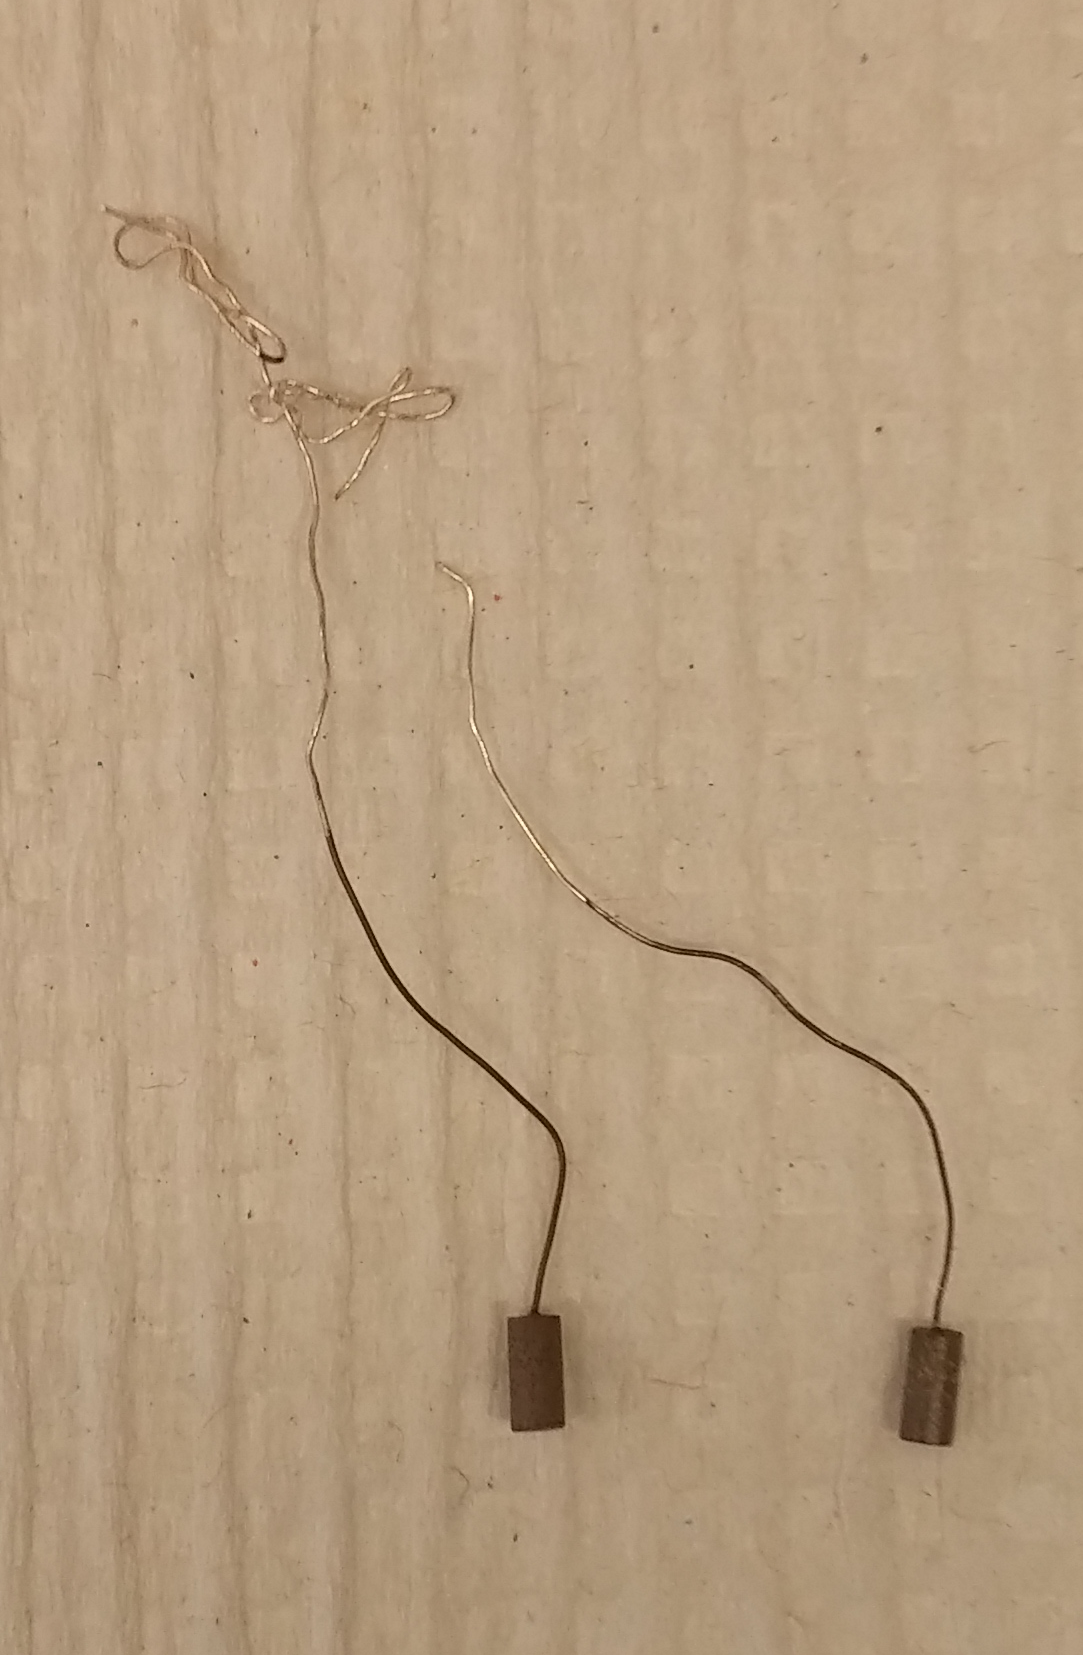
\includegraphics[height=2.25cm]{photo/electrodes.png}
%  		\hspace{.35cm}
% 	\end{center}

\end{frame}

%%%%%%%%%%%%%%%%%%%%%%%%%%%%%%%%%%%%%%%%%%%%%%%%%%%%%%%%%%%%%%%%%%%%%%%%%%%%%%%%%%%%%%%%%%%%%%%%%%%%%%%%%%%%%%%%%%%%%%%%%%%%
% Resistive pulse background---electrostatic boundary conditions
%%%%%%%%%%%%%%%%%%%%%%%%%%%%%%%%%%%%%%%%%%%%%%%%%%%%%%%%%%%%%%%%%%%%%%%%%%%%%%%%%%%%%%%%%%%%%%%%%%%%%%%%%%%%%%%%%%%%%%%%%%%%

\begin{frame}[c]{Resistive pulse sensing}
	{\centering
		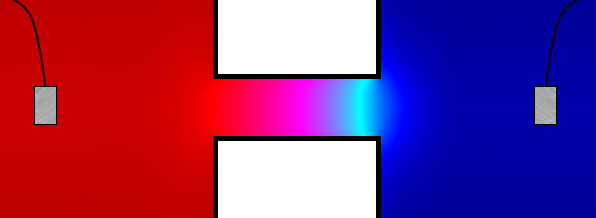
\includegraphics[width=0.9\paperwidth]{comsol/voltage.png}
		\par
	}
\end{frame}

%%%%%%%%%%%%%%%%%%%%%%%%%%%%%%%%%%%%%%%%%%%%%%%%%%%%%%%%%%%%%%%%%%%%%%%%%%%%%%%%%%%%%%%%%%%%%%%%%%%%%%%%%%%%%%%%%%%%%%%%%%%%
% Resistive pulse background---electrostatic boundary conditions
%%%%%%%%%%%%%%%%%%%%%%%%%%%%%%%%%%%%%%%%%%%%%%%%%%%%%%%%%%%%%%%%%%%%%%%%%%%%%%%%%%%%%%%%%%%%%%%%%%%%%%%%%%%%%%%%%%%%%%%%%%%%

\begin{frame}[c]{Resistive pulse sensing---electrostatic boundary conditions}
	{\centering
		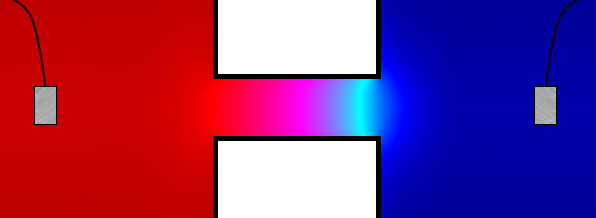
\includegraphics[width=0.9\paperwidth]{comsol/voltage.png}
		\par
	}
\end{frame}


%%%%%%%%%%%%%%%%%%%%%%%%%%%%%%%%%%%%%%%%%%%%%%%%%%%%%%%%%%%%%%%%%%%%%%%%%%%%%%%%%%%%%%%%%%%%%%%%%%%%%%%%%%%%%%%%%%%%%%%%%%%%
% Resistive pulse background---ion transport
%%%%%%%%%%%%%%%%%%%%%%%%%%%%%%%%%%%%%%%%%%%%%%%%%%%%%%%%%%%%%%%%%%%%%%%%%%%%%%%%%%%%%%%%%%%%%%%%%%%%%%%%%%%%%%%%%%%%%%%%%%%%

\tikzset{cross/.style={cross out, draw=black, minimum size=2*(#1-\pgflinewidth), inner sep=0pt, outer sep=0pt},
%default radius will be 1pt. 
cross/.default={1pt}}



\begin{frame}[c]{Resistive pulse sensing---ion transport}
	\begin{itemize}
		\item Ion transport is driven by \textbf{diffusion}, \textbf{convection}, and \textbf{electric migration}
		\item \underline{Diffusion}: Average flow of ions from high to low concentration
		\item \underline{Convection}: Ions move with the fluid/solvent
		\item \underline{Electrical migration}: Ions move in electric field
	\end{itemize}
	\only<1>{
		$$ \vec{J}_{i}=\underbrace{z_{i}eD_{i}\nabla c_{i}}_{\mathrm{diffusion}}+\overbrace{z_{i}ec_{i}\vec{u}}^{\mathrm{convection}}+\underbrace{z_{i}ec_{i}\mu_{i}\vec{E}}_{\mathrm{migration}} $$
	}
	\only<2>{
		$$ \vec{J}_{i}=\underbrace{\xcancel{z_{i}eD_{i}\nabla c_{i}}}_{\mathrm{diffusion}}+\overbrace{\xcancel{z_{i}ec_{i}\vec{u}}}^{\mathrm{convection}}+\underbrace{z_{i}ec_{i}\mu_{i}\vec{E}}_{\mathrm{migration}} $$
	}
	
	$$ I=\sum_{i}\iint_{S}\vec{J_{i}}\cdot \hat{n}dS $$
	
	% xs over two terms in equation
	\onslide<2>{
		\begin{tikzpicture}[]
			\draw(300,25) node[cross=10pt,red] {};
			\draw(1,0) node[cross=10pt,red] {};
		\end{tikzpicture}
	}

\end{frame}




%%%%%%%%%%%%%%%%%%%%%%%%%%%%%%%%%%%%%%%%%%%%%%%%%%%%%%%%%%%%%%%%%%%%%%%%%%%%%%%%%%%%%%%%%%%%%%%%%%%%%%%%%%%%%%%%%%%%%%%%%%%%
% Rods title slide
%%%%%%%%%%%%%%%%%%%%%%%%%%%%%%%%%%%%%%%%%%%%%%%%%%%%%%%%%%%%%%%%%%%%%%%%%%%%%%%%%%%%%%%%%%%%%%%%%%%%%%%%%%%%%%%%%%%%%%%%%%%%


\begin{frame}[c]{}
	\begin{center}
		\textbf{Resistive pulse sensing of high-aspect ratio particles}
	\end{center}
\end{frame}




%%%%%%%%%%%%%%%%%%%%%%%%%%%%%%%%%%%%%%%%%%%%%%%%%%%%%%%%%%%%%%%%%%%%%%%%%%%%%%%%%%%%%%%%%%%%%%%%%%%%%%%%%%%%%%%%%%%%%%%%%%%%
% Rods motivation slide
%%%%%%%%%%%%%%%%%%%%%%%%%%%%%%%%%%%%%%%%%%%%%%%%%%%%%%%%%%%%%%%%%%%%%%%%%%%%%%%%%%%%%%%%%%%%%%%%%%%%%%%%%%%%%%%%%%%%%%%%%%%%


\begin{frame}[c]{High-aspect ratio resistive pulse sensing---motivation}
 	\begin{itemize}
 		\item Aspherical particles are ubiquitous in biology---e.g., many viruses and bacteria are approximately rod-shaped
 	\end{itemize}


	\begin{columns}[t]
		\begin{column}[T]{2.5in}
			{\centering
				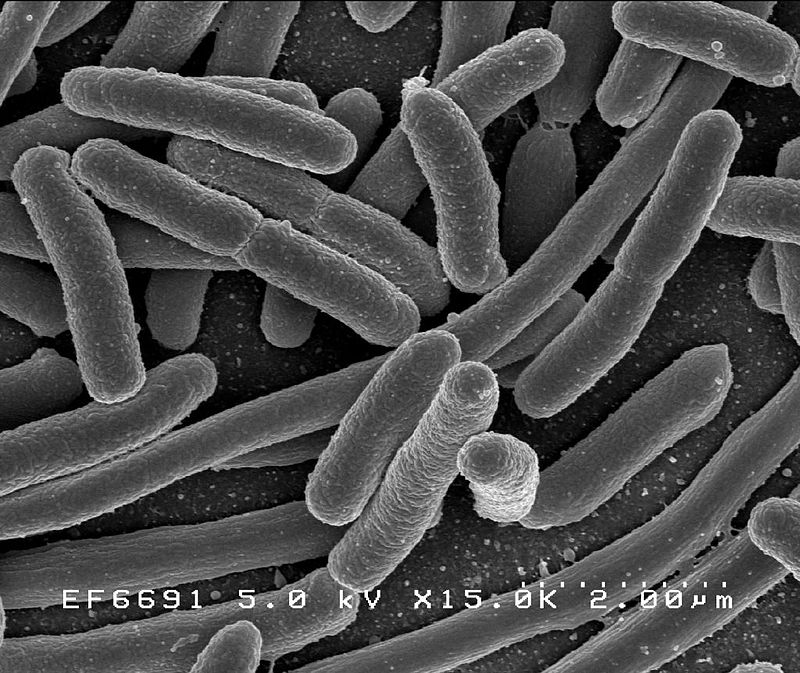
\includegraphics[height=2.25cm]{ecoli} \\
				e. coli \\
				$L\sim \SI{2}{\mu m}$ \\
				\par
			}
		\end{column}
		
		
		\begin{column}[T]{2.5in}
			{\centering
				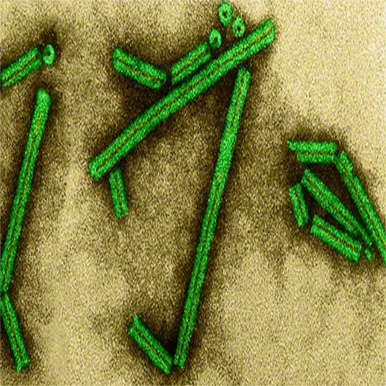
\includegraphics[height=2.25cm]{tobaccomosaicvirus} \\
				tobacco mosaic virus \\
				$L\sim \SI{300}{nm}$ \\
				\par
			}
		\end{column}
	

	\end{columns}

	\begin{itemize}
		\item The ability to measure particle shape is highly desirable for sensing applications
 		\item How can we extend RP sensing to measure length in addition to volume?
 	\end{itemize}
	

\end{frame}




%%%%%%%%%%%%%%%%%%%%%%%%%%%%%%%%%%%%%%%%%%%%%%%%%%%%%%%%%%%%%%%%%%%%%%%%%%%%%%%%%%%%%%%%%%%%%%%%%%%%%%%%%%%%%%%%%%%%%%%%%%%%
% Resistive pulse in non-constant width pores
%%%%%%%%%%%%%%%%%%%%%%%%%%%%%%%%%%%%%%%%%%%%%%%%%%%%%%%%%%%%%%%%%%%%%%%%%%%%%%%%%%%%%%%%%%%%%%%%%%%%%%%%%%%%%%%%%%%%%%%%%%%%

\begin{frame}[c]{Resistive pulse in non-constant width pores}
	\begin{itemize}
		\item Consider the RP amplitude for translocation through non-uniform pores
	\end{itemize}
	$$ \Delta R\left(z'\right)=\frac{\rho}{\pi}\left[\int_{z=z'}^{z=z'+l_{p}}\left(\frac{1}{r_{P}^{2}\left(z\right)-s_{p}^{2}\left(z\right)}-\frac{1}{r_{P}\left(z\right)^{2}}\right)dz\right] $$
	\begin{itemize}
		\item RP amplitude is a function of the pore geometry \textbf{local to the particle's position}
		\item Particles map the interior of the pore during translocation with their RP signal!
	\end{itemize}
	
	{\centering
		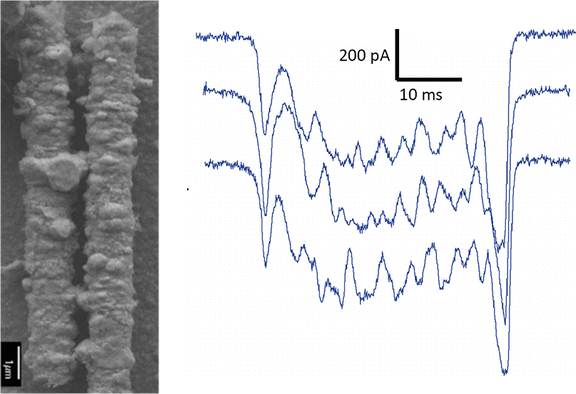
\includegraphics[width=2in]{particlesreveal.png} \\
		\par
	}

	
\end{frame}


%%%%%%%%%%%%%%%%%%%%%%%%%%%%%%%%%%%%%%%%%%%%%%%%%%%%%%%%%%%%%%%%%%%%%%%%%%%%%%%%%%%%%%%%%%%%%%%%%%%%%%%%%%%%%%%%%%%%%%%%%%%%
% RP signal resolution
%%%%%%%%%%%%%%%%%%%%%%%%%%%%%%%%%%%%%%%%%%%%%%%%%%%%%%%%%%%%%%%%%%%%%%%%%%%%%%%%%%%%%%%%%%%%%%%%%%%%%%%%%%%%%%%%%%%%%%%%%%%%

\begin{frame}[c]{RP signal resolution}
	
	\vspace{-.1in}
	\begin{itemize}
		\item Particles map pore interiors with a length-dependent resolution
		\item If a particle has length smaller than the characteristic length scale of channel irregularities, the produced signal is a high-resolution mapping
		\item Particles with lengths longer than characteristic length scale of channel irregularities produce low-resolution mappings
	\end{itemize}
	
	
	
	\begin{columns}[t]
		
	
		\begin{column}[T]{2.25in}
			{\centering
				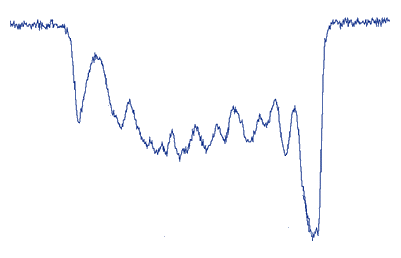
\includegraphics[height=1in]{plain_signal.png} \\
				Short particle \\
			}
		\end{column}
		  
		\begin{column}[T]{2.25in}
			{\centering
				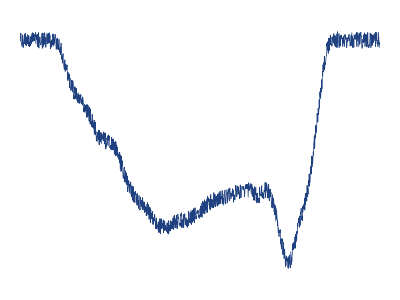
\includegraphics[height=1.in,width=2in]{mystery_plain_signal_3.png} \\
				Long particle (simulated) \\
			}
		\end{column}

	\end{columns}
	\vspace{.2in}
	\textcolor{negativered}{\textbf{Can we use this knowledge to measure particle length???}}

	%$$ \Delta R\left(z'\right)=\frac{\rho}{\pi}\left[\int_{z=z'}^{z=z'+l_{p}}\left(\frac{1}{r_{P}^{2}\left(z\right)-s_{p}^{2}\left(z\right)}-\frac{1}{r_{P}^{2}\left(z\right)}\right)dz\right] $$

	
	
	
	

\end{frame}


%%%%%%%%%%%%%%%%%%%%%%%%%%%%%%%%%%%%%%%%%%%%%%%%%%%%%%%%%%%%%%%%%%%%%%%%%%%%%%%%%%%%%%%%%%%%%%%%%%%%%%%%%%%%%%%%%%%%%%%%%%%%
% Qualitative length comparison
%%%%%%%%%%%%%%%%%%%%%%%%%%%%%%%%%%%%%%%%%%%%%%%%%%%%%%%%%%%%%%%%%%%%%%%%%%%%%%%%%%%%%%%%%%%%%%%%%%%%%%%%%%%%%%%%%%%%%%%%%%%%

\begin{frame}[c]{Qualitative length comparison}
	\vspace{.3in}
	\begin{picture}(0,0)(0,0)
		\put(0,-25)
		{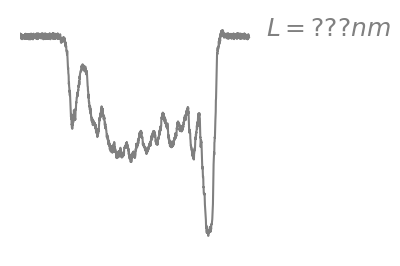
\includegraphics[width=3.75cm]{mystery_plain_signal_2.png}}
		\put(0,-125)
		{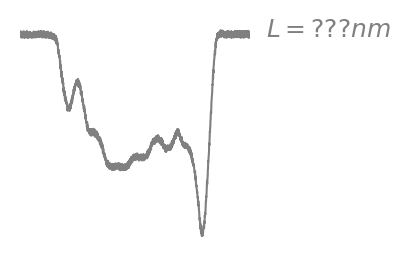
\includegraphics[width=3.75cm]{mystery_plain_signal.png}}
		\put(200,-125)
		{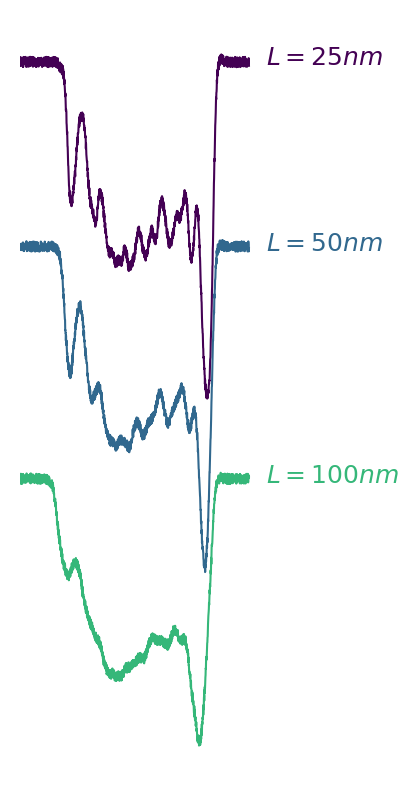
\includegraphics[height=7cm]{plain_signals_smoothed.png}}
	\end{picture}
	
	\begin{tikzpicture}[overlay, x=1cm,y=1cm]
		% Coordinates
		\coordinate (x1) at (2.5, -2.5) ;
		\coordinate (x2) at (5.5, -2.5) ;
		\coordinate (x3) at (5.5, -.5) ;
		\coordinate (x4) at (7.25, -.5) ;
		
		
		\coordinate (x5) at (2.5, 1.) ;
		\coordinate (x6) at (5.5, 1.) ;
		\coordinate (x7) at (5.5, 2.95) ;
		\coordinate (x8) at (7.25, 2.95) ;

		% Text hack
		\node[right] (mag) at (0.25,3.5) {\footnotesize\textcolor{porestatsblack}{Unidentified particles}};
		\node[right] (mag) at (7.25,3.5) {\footnotesize\textcolor{porestatsblack}{Tracer particles}};


		    		    
		% Arrow
		\path[draw=gray1,thick,->] (x1) to[straight] (x2) to[straight] (x3) to[straight] (x4);
		\path[draw=gray1,thick,->] (x5) to[straight] (x6) to[straight] (x7) to[straight] (x8);


			
	\end{tikzpicture}
	

\end{frame}


%%%%%%%%%%%%%%%%%%%%%%%%%%%%%%%%%%%%%%%%%%%%%%%%%%%%%%%%%%%%%%%%%%%%%%%%%%%%%%%%%%%%%%%%%%%%%%%%%%%%%%%%%%%%%%%%%%%%%%%%%%%%
% Quantitative length measurement
%%%%%%%%%%%%%%%%%%%%%%%%%%%%%%%%%%%%%%%%%%%%%%%%%%%%%%%%%%%%%%%%%%%%%%%%%%%%%%%%%%%%%%%%%%%%%%%%%%%%%%%%%%%%%%%%%%%%%%%%%%%%

\begin{frame}[c]{Reexpressing the RP amplitude of a long particle in terms of shorter particles}
	
	
	{\footnotesize
	Because resistances add in series, we can express the RP amplitude of a long particle as a sum over the RP amplitudes of shorter particles
	}
	
	
	{\scriptsize
		\begin{equation*}
			\begin{split}
				\Delta R_{l}\left(z\right) &= \frac{\rho}{\pi}\left[\int_{z}^{z+l_{p}}\left(\frac{1}{r_{P}^{2}\left(z'\right)-s_{p}^{2}\left(z'\right)}-\frac{1}{r_{P}^{2}\left(z'\right)}\right)dz'\right] \\
				%&= \frac{\rho}{\pi}\left[\int_{z}^{z+l_{s}}\left(\frac{1}{r_{P}^{2}\left(z'\right)-%s_{p}^{2}\left(z'\right)}-\frac{1}{r_{P}^{2}\left(z'\right)}\right)dz'\right. \\
				%&+ \int_{z+l_{s}}^{z+2l_{s}}\left(\frac{1}{r_{P}^{2}\left(z'\right)-s_{p}^{2}\left(z'\right)}-\frac{1}%{r_{P}^{2}\left(z'\right)}\right)dz + ...\\
				%&+ \left.\int_{z+\left(n-1\right)l_{s}}^{z+nl_{s}}\left(\frac{1}{r_{P}^{2}\left(z'\right)-%s_{p}^{2}\left(z'\right)}-\frac{1}{r_{P}^{2}\left(z'\right)}\right)dz'\right] \\
				&= \sum_{i=0}^{n-1}\frac{\rho}{\pi}\left[\int_{z+il_{s}}^{z+\left(i+1\right)l_{s}}\left(\frac{1}{r^{2}_{P}\left(z'\right)-s^{2}_{p}\left(z'\right)}-\frac{1}{r_{P}^{2}\left(z'\right)}\right)dz'\right] \\
				&= \sum_{i=0}^{n-1}\Delta R_{s}\left(z+il_{s}\right)
			\end{split}
		\end{equation*}
	}
		
	{\footnotesize In terms of the measured RP signal, we relate resistance to current via }
		
	{\scriptsize \[ \frac{\Delta R}{R_{0}}=\frac{\Delta I}{I_{p}} \]}
	


		



\end{frame}




%%%%%%%%%%%%%%%%%%%%%%%%%%%%%%%%%%%%%%%%%%%%%%%%%%%%%%%%%%%%%%%%%%%%%%%%%%%%%%%%%%%%%%%%%%%%%%%%%%%%%%%%%%%%%%%%%%%%%%%%%%%%
% Quantitative length measurement
%%%%%%%%%%%%%%%%%%%%%%%%%%%%%%%%%%%%%%%%%%%%%%%%%%%%%%%%%%%%%%%%%%%%%%%%%%%%%%%%%%%%%%%%%%%%%%%%%%%%%%%%%%%%%%%%%%%%%%%%%%%%

\begin{frame}[c]{Quantitative length measurement}
	

	{\footnotesize
		Reexpressing the amplitude of long particles in terms of amplitude of short particles suggests a protocol for measuring length \\
		\begin{enumerate}
			\item We transform the signals of short particles via a moving average to simulate the signals of longer particles \\
			\item Then, we compare an unknown particle's signal with each of the simulated signals of the shorter particle \\
			\item The comparison with the greatest similarity yields the length of the particle
		\end{enumerate}
	}

\end{frame}



%%%%%%%%%%%%%%%%%%%%%%%%%%%%%%%%%%%%%%%%%%%%%%%%%%%%%%%%%%%%%%%%%%%%%%%%%%%%%%%%%%%%%%%%%%%%%%%%%%%%%%%%%%%%%%%%%%%%%%%%%%%%
% Quantitative length measurement
%%%%%%%%%%%%%%%%%%%%%%%%%%%%%%%%%%%%%%%%%%%%%%%%%%%%%%%%%%%%%%%%%%%%%%%%%%%%%%%%%%%%%%%%%%%%%%%%%%%%%%%%%%%%%%%%%%%%%%%%%%%%

\begin{frame}[c]{Quantitative length measurement---parametric signal transformation}
	\begin{columns}[t]
	
		\begin{column}[T]{2.25in}
			{\centering
				Single transformation \\
				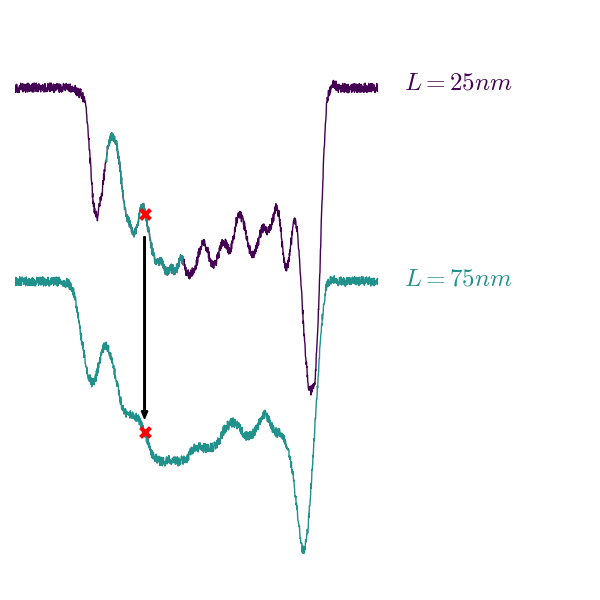
\includegraphics[width=2.25in]{moving_average_process.png} \\
				\par
			}
		\end{column}
		\hfill
		\begin{column}[T]{2.25in}
			{\centering
				Multiple length transformations \\
				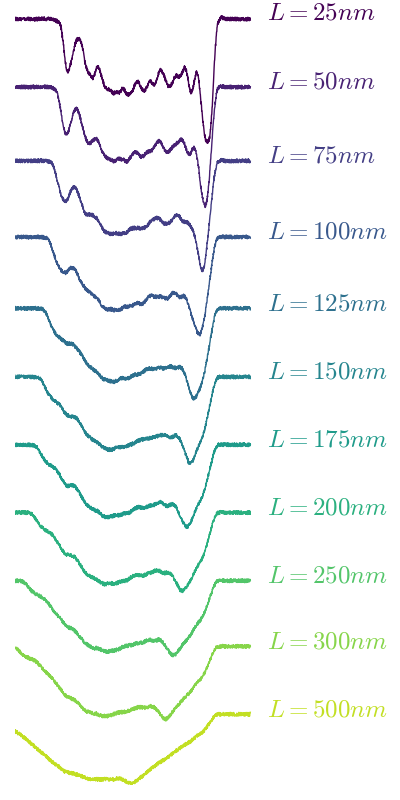
\includegraphics[width=1.25in]{many_plain_signals_smoothed.png} \\
				\par
			}
		\end{column}

	\end{columns}
	


\end{frame}



%%%%%%%%%%%%%%%%%%%%%%%%%%%%%%%%%%%%%%%%%%%%%%%%%%%%%%%%%%%%%%%%%%%%%%%%%%%%%%%%%%%%%%%%%%%%%%%%%%%%%%%%%%%%%%%%%%%%%%%%%%%%
% Quantitative length measurement
%%%%%%%%%%%%%%%%%%%%%%%%%%%%%%%%%%%%%%%%%%%%%%%%%%%%%%%%%%%%%%%%%%%%%%%%%%%%%%%%%%%%%%%%%%%%%%%%%%%%%%%%%%%%%%%%%%%%%%%%%%%%

\begin{frame}[c]{Quantitative length measurement---signal similarity measure}
	\vspace{-.1in}
	\begin{columns}[t]
	
		\begin{column}[T]{2.25in}
			{\centering
				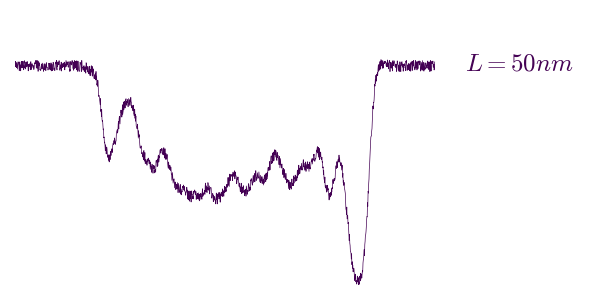
\includegraphics[width=2in]{mystery_signal_7.png} \\
				\par
			}
		\end{column}
		
		\begin{column}[T]{2.25in}
			{\centering
				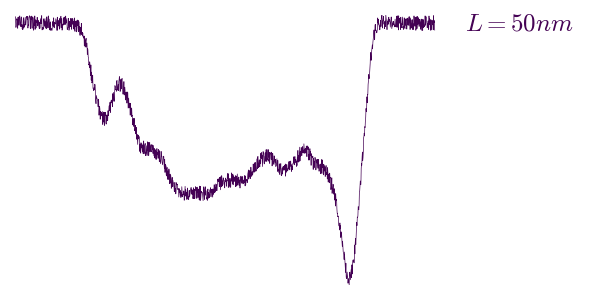
\includegraphics[width=2in]{transformed_signal.png} \\
				\par
			}
		\end{column}

	\end{columns}

	\vspace{.2in}	
	
	\begin{columns}[t]
	
		\begin{column}[T]{\paperwidth/3}
			{\centering
				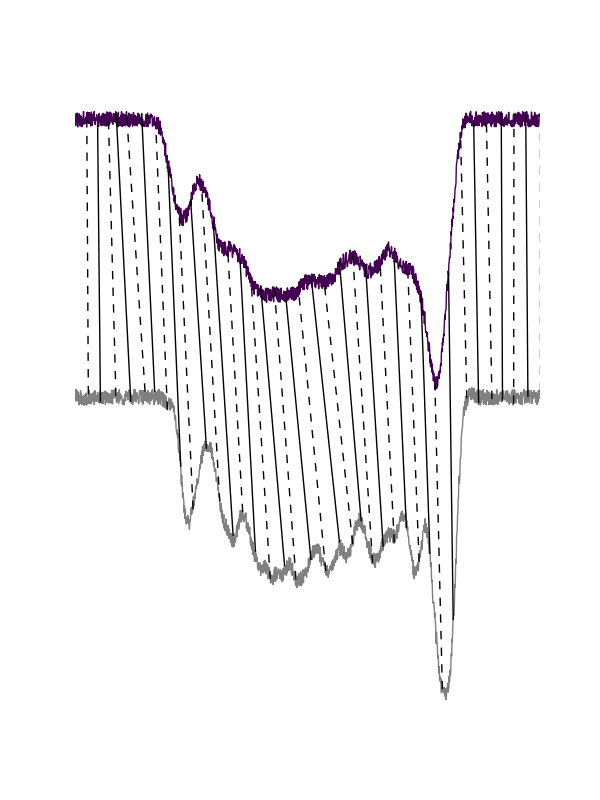
\includegraphics[width=1.25in]{dtw_matching.png} \\
				\par
			}
		\end{column}
		
		\begin{column}[T]{\paperwidth/3}
			{\centering
				\vspace{.2in}
				{\scriptsize \[\mathrm{Cost}=\sum_{\left(i,i'\right)}\left[\left(\frac{\Delta I}{I_{p}}\right)_{i}-\left(\frac{\Delta I}{I_{p}}\right)_{i'}\right] \] } \\
				\par
			}
		\end{column}
		
		\begin{column}[T]{\paperwidth/3}
			{\centering
				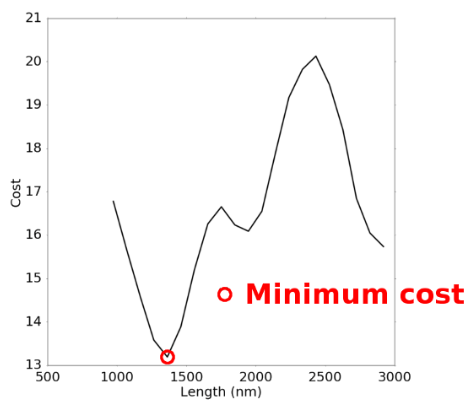
\includegraphics[width=1.5in]{cost_minimization.png} \\
				\par
			}
		\end{column}

	\end{columns}
	


\end{frame}





%%%%%%%%%%%%%%%%%%%%%%%%%%%%%%%%%%%%%%%%%%%%%%%%%%%%%%%%%%%%%%%%%%%%%%%%%%%%%%%%%%%%%%%%%%%%%%%%%%%%%%%%%%%%%%%%%%%%%%%%%%%%
% Length measurement experimental platform
%%%%%%%%%%%%%%%%%%%%%%%%%%%%%%%%%%%%%%%%%%%%%%%%%%%%%%%%%%%%%%%%%%%%%%%%%%%%%%%%%%%%%%%%%%%%%%%%%%%%%%%%%%%%%%%%%%%%%%%%%%%%

\begin{frame}[c]{Length measurement experimental test}
	\textcolor{negativered}{Can we experimentally implement and test the length measurement protocol?} \\
	\begin{itemize}
		\item Experiments were conducted with single pores etched into PET membranes $\left(D\sim\SI{750}{nm}, L=\SI{12}{\mu m}\right)$
		\item Three types of particles were tested
		\begin{itemize}
			\item $280$ and $\SI{400}{nm}$ polystyrene beads  (`spheres')
			\item $\SI{590}{nm}$ rods (`short rods')
			\item $\SI{1920}{nm}$ rods (`long rods')
		\end{itemize}
	\end{itemize}
	
	\begin{columns}[t]
		\begin{column}[T]{2.25in}
			{\centering
				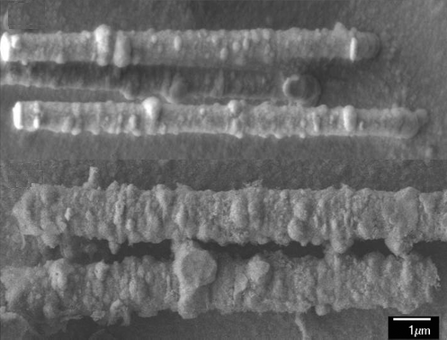
\includegraphics[height=0.75in]{PET.png} \\
				PET pore metal replica \\
				\par
			}
		\end{column}
		
		\begin{column}[T]{2.25in}
			{\centering
				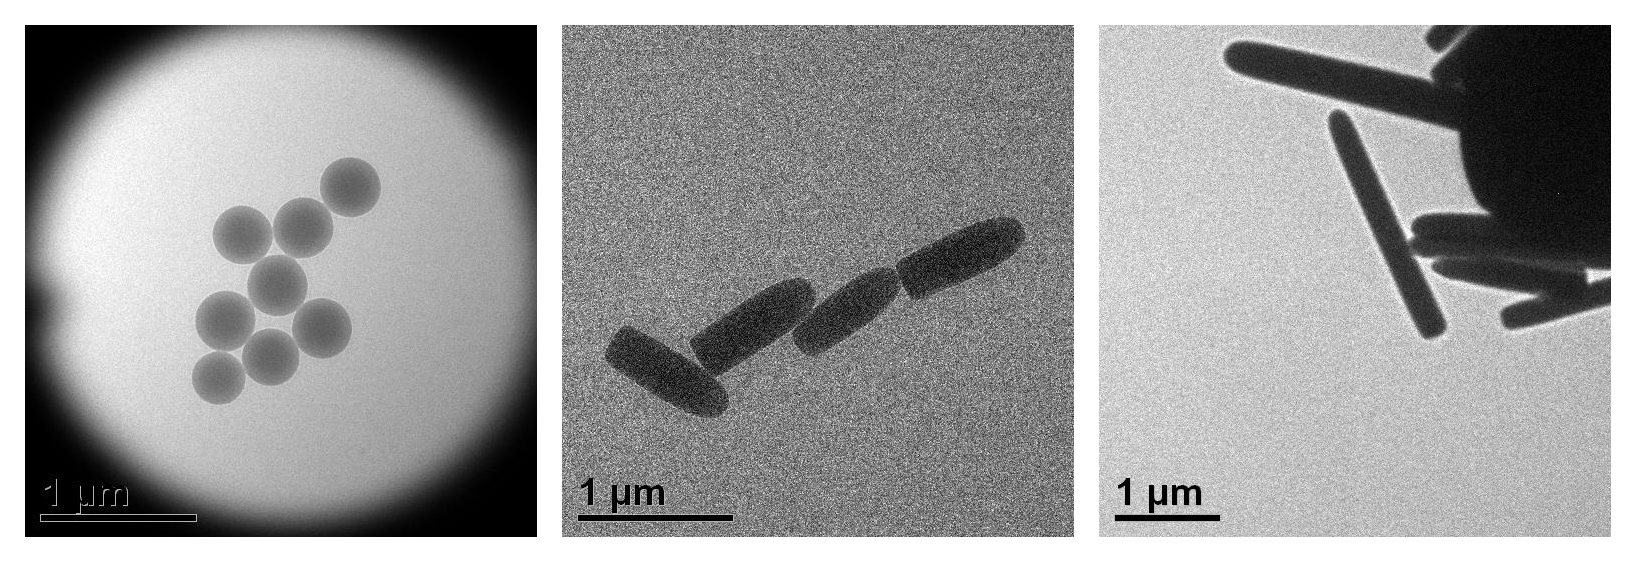
\includegraphics[height=0.75in]{particles.png} \\
				Nanoparticles \\
				\par				
			}
		\end{column}

	\end{columns}



\end{frame}



%%%%%%%%%%%%%%%%%%%%%%%%%%%%%%%%%%%%%%%%%%%%%%%%%%%%%%%%%%%%%%%%%%%%%%%%%%%%%%%%%%%%%%%%%%%%%%%%%%%%%%%%%%%%%%%%%%%%%%%%%%%%
% Length measurement experimental platform
%%%%%%%%%%%%%%%%%%%%%%%%%%%%%%%%%%%%%%%%%%%%%%%%%%%%%%%%%%%%%%%%%%%%%%%%%%%%%%%%%%%%%%%%%%%%%%%%%%%%%%%%%%%%%%%%%%%%%%%%%%%%

\begin{frame}[c]{Particles to scale}
	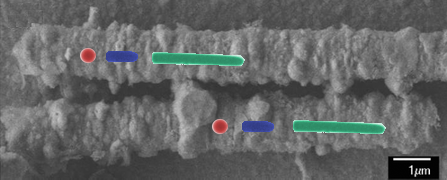
\includegraphics[width=4.5in]{particles_real_size.png}
\end{frame}

%%%%%%%%%%%%%%%%%%%%%%%%%%%%%%%%%%%%%%%%%%%%%%%%%%%%%%%%%%%%%%%%%%%%%%%%%%%%%%%%%%%%%%%%%%%%%%%%%%%%%%%%%%%%%%%%%%%%%%%%%%%%
% Results---raw data
%%%%%%%%%%%%%%%%%%%%%%%%%%%%%%%%%%%%%%%%%%%%%%%%%%%%%%%%%%%%%%%%%%%%%%%%%%%%%%%%%%%%%%%%%%%%%%%%%%%%%%%%%%%%%%%%%%%%%%%%%%%%

\begin{frame}[c]{Results---raw data}

	{\centering
		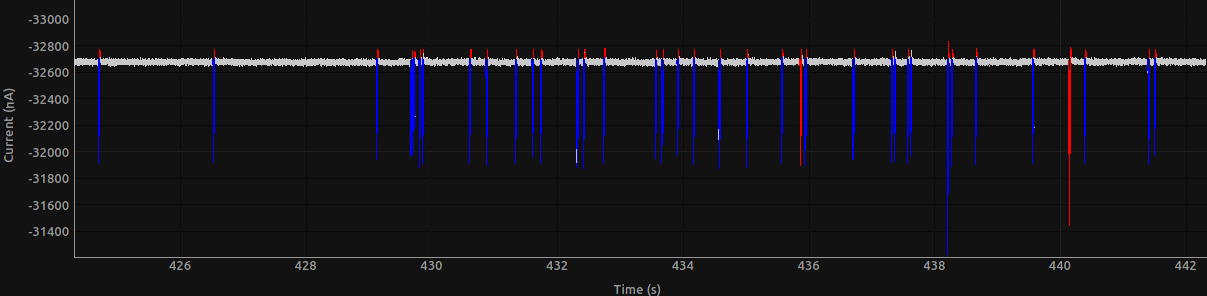
\includegraphics[width=3.75in]{experiment_timeseries.png} \\
		Resistive pulse time series \\
		\par
	}
	
	\begin{columns}[t]
		\begin{column}[T]{2.25in}
			{\centering
				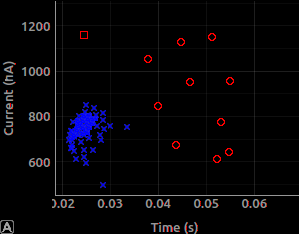
\includegraphics[height=1.25in]{experiment_scatter.png} \\
				Amplitude-duration scatter
				\par
			}
		\end{column}
		
		\begin{column}[T]{2.25in}
			{\centering
				\includegraphics[height=1.25in]{experiment_singleevent.png} \\
				Raw event \\
				\par
			}
		\end{column}

	\end{columns}
	
\end{frame}






%%%%%%%%%%%%%%%%%%%%%%%%%%%%%%%%%%%%%%%%%%%%%%%%%%%%%%%%%%%%%%%%%%%%%%%%%%%%%%%%%%%%%%%%%%%%%%%%%%%%%%%%%%%%%%%%%%%%%%%%%%%%
% Results---PET21---Raw
%%%%%%%%%%%%%%%%%%%%%%%%%%%%%%%%%%%%%%%%%%%%%%%%%%%%%%%%%%%%%%%%%%%%%%%%%%%%%%%%%%%%%%%%%%%%%%%%%%%%%%%%%%%%%%%%%%%%%%%%%%%%
 
 \begin{frame}[c]{Results---sphere, short rod, and long rod events}
 	\includegraphics[width=4.25in]{PET21_raw.png}
 \end{frame}

 
% %%%%%%%%%%%%%%%%%%%%%%%%%%%%%%%%%%%%%%%%%%%%%%%%%%%%%%%%%%%%%%%%%%%%%%%%%%%%%%%%%%%%%%%%%%%%%%%%%%%%%%%%%%%%%%%%%%%%%%%%%%%%
% % Results---PET21---Smoothed
% %%%%%%%%%%%%%%%%%%%%%%%%%%%%%%%%%%%%%%%%%%%%%%%%%%%%%%%%%%%%%%%%%%%%%%%%%%%%%%%%%%%%%%%%%%%%%%%%%%%%%%%%%%%%%%%%%%%%%%%%%%%%
% 
% \begin{frame}[c]{Results---PET21 averaged events}
% 	\includegraphics[width=4.5in]{PET21_averaged.png}
% \end{frame}




%%%%%%%%%%%%%%%%%%%%%%%%%%%%%%%%%%%%%%%%%%%%%%%%%%%%%%%%%%%%%%%%%%%%%%%%%%%%%%%%%%%%%%%%%%%%%%%%%%%%%%%%%%%%%%%%%%%%%%%%%%%%
% Results---PET7---Raw and averaged event comparison
%%%%%%%%%%%%%%%%%%%%%%%%%%%%%%%%%%%%%%%%%%%%%%%%%%%%%%%%%%%%%%%%%%%%%%%%%%%%%%%%%%%%%%%%%%%%%%%%%%%%%%%%%%%%%%%%%%%%%%%%%%%%

\begin{frame}[c]{Results---Qualitative event comparison}
	{\centering
		\includegraphics[width=3.5in]{PETevents.png} \\
		\textcolor{negativered}{The averaging process produces signals that are qualitatively similar to the observed signals of longer particles}
		\par
	}
\end{frame}



%%%%%%%%%%%%%%%%%%%%%%%%%%%%%%%%%%%%%%%%%%%%%%%%%%%%%%%%%%%%%%%%%%%%%%%%%%%%%%%%%%%%%%%%%%%%%%%%%%%%%%%%%%%%%%%%%%%%%%%%%%%%
% Results---PET7---Raw and smoothed
%%%%%%%%%%%%%%%%%%%%%%%%%%%%%%%%%%%%%%%%%%%%%%%%%%%%%%%%%%%%%%%%%%%%%%%%%%%%%%%%%%%%%%%%%%%%%%%%%%%%%%%%%%%%%%%%%%%%%%%%%%%%

\begin{frame}[c]{Results---Quantitative event comparison}
	{\centering
		\includegraphics[width=2.75in]{dtwfit.png} \\
		\textcolor{negativered}{Quantitative measurement of particle length yields a distribution closely matching the actual distribution of lengths!}
		\par
	}
\end{frame}



%%%%%%%%%%%%%%%%%%%%%%%%%%%%%%%%%%%%%%%%%%%%%%%%%%%%%%%%%%%%%%%%%%%%%%%%%%%%%%%%%%%%%%%%%%%%%%%%%%%%%%%%%%%%%%%%%%%%%%%%%%%%
% Future work
%%%%%%%%%%%%%%%%%%%%%%%%%%%%%%%%%%%%%%%%%%%%%%%%%%%%%%%%%%%%%%%%%%%%%%%%%%%%%%%%%%%%%%%%%%%%%%%%%%%%%%%%%%%%%%%%%%%%%%%%%%%%

\begin{frame}[c]{Future work}
	Some things left for the future:
	\begin{enumerate}
		\item Test robustness of quantitative length measurement
		\item Run length measurement protocol on particles of various unknown lengths, test results
		\item Reduce system scale: Test length measurement protocol with fabricated planar nanochannels with controlled geometries
	\end{enumerate}
\end{frame}



%%%%%%%%%%%%%%%%%%%%%%%%%%%%%%%%%%%%%%%%%%%%%%%%%%%%%%%%%%%%%%%%%%%%%%%%%%%%%%%%%%%%%%%%%%%%%%%%%%%%%%%%%%%%%%%%%%%%%%%%%%%%
% RP-IM title slide
%%%%%%%%%%%%%%%%%%%%%%%%%%%%%%%%%%%%%%%%%%%%%%%%%%%%%%%%%%%%%%%%%%%%%%%%%%%%%%%%%%%%%%%%%%%%%%%%%%%%%%%%%%%%%%%%%%%%%%%%%%%%


\begin{frame}[c]{}
	\begin{center}
		\textbf{Hybrid imaging-resistive pulse measurements in microfluidic channels}
	\end{center}
\end{frame}



%%%%%%%%%%%%%%%%%%%%%%%%%%%%%%%%%%%%%%%%%%%%%%%%%%%%%%%%%%%%%%%%%%%%%%%%%%%%%%%%%%%%%%%%%%%%%%%%%%%%%%%%%%%%%%%%%%%%%%%%%%%%
% RP-IM motivation 1
%%%%%%%%%%%%%%%%%%%%%%%%%%%%%%%%%%%%%%%%%%%%%%%%%%%%%%%%%%%%%%%%%%%%%%%%%%%%%%%%%%%%%%%%%%%%%%%%%%%%%%%%%%%%%%%%%%%%%%%%%%%%


\begin{frame}[c]{Motivation 1}
	
	In an RP experiment, the usual parameters measured are amplitude and duration, which can relate to particle's volume, charge, etc. \\
	
	But, the equations which relate the RP signal to the physical observable are only accurate under restricting conditions that are seldom met in experimental systems \\
	
	For instance, spheroids moving along the axis of an infinitely long cylinder \\
	
	\vspace{.25in}
	
	{\centering
		Sphere \hspace{.2in} $\frac{\Delta I}{I_{p}}=\frac{d^{3}}{D^{2}L}\left[1-0.8\left(\frac{d}{D}\right)^{3}\right]^{-1}$ \\
		\vspace{.1in}
		Ellipsoid \hspace{.2in} $\frac{\Delta I}{I_{p}}=\left[f_{\perp}+\left(f_{\parallel}-f_{\perp}\right)\cos^{2}\alpha\right]\frac{v}{V}$ \\
	}
	
		 
 	%\begin{equation}
 	%	\frac{\Delta I}{I_{p}}=\frac{d^{3}}{D^{2}L}\left[1-0.8\left(\frac{d}{D}\right)^{3}\right]^{-1}
 	%\end{equation}



\end{frame}



%%%%%%%%%%%%%%%%%%%%%%%%%%%%%%%%%%%%%%%%%%%%%%%%%%%%%%%%%%%%%%%%%%%%%%%%%%%%%%%%%%%%%%%%%%%%%%%%%%%%%%%%%%%%%%%%%%%%%%%%%%%%
% RP-IM motivation 2
%%%%%%%%%%%%%%%%%%%%%%%%%%%%%%%%%%%%%%%%%%%%%%%%%%%%%%%%%%%%%%%%%%%%%%%%%%%%%%%%%%%%%%%%%%%%%%%%%%%%%%%%%%%%%%%%%%%%%%%%%%%%


\begin{frame}[c]{Motivation 2}
	
	
	
	In reality, the experimental set up can never be constrained to this degree
	
	Some confounding factors include
	
	\begin{itemize}
		\item Entrance effects in low or medium aspect ratio pores
		\item Non-spheroidal particles, rotational effects
		\item Off-axis translocation
	\end{itemize}
	
	The influence of each of these effects on the RP signal is difficult to measure

\end{frame}



%%%%%%%%%%%%%%%%%%%%%%%%%%%%%%%%%%%%%%%%%%%%%%%%%%%%%%%%%%%%%%%%%%%%%%%%%%%%%%%%%%%%%%%%%%%%%%%%%%%%%%%%%%%%%%%%%%%%%%%%%%%%
% RP-IM motivation 3
%%%%%%%%%%%%%%%%%%%%%%%%%%%%%%%%%%%%%%%%%%%%%%%%%%%%%%%%%%%%%%%%%%%%%%%%%%%%%%%%%%%%%%%%%%%%%%%%%%%%%%%%%%%%%%%%%%%%%%%%%%%%


\begin{frame}[c]{Motivation 3}
	
	What if we could \textit{see} what is happening during a resistive pulse experiment? Then we could determine the influence of these confounding factors during the event translocation \\
	
	\vspace{.2in}
	
	For instance, we could directly observe the effect of off-axis translocation on the resistive pulse signal \\
	
	\vspace{.2in}
	
	The results would generalize to other resistive pulse experiments and lead to better interpretability of the resistive pulse signals! \\

\end{frame}



%%%%%%%%%%%%%%%%%%%%%%%%%%%%%%%%%%%%%%%%%%%%%%%%%%%%%%%%%%%%%%%%%%%%%%%%%%%%%%%%%%%%%%%%%%%%%%%%%%%%%%%%%%%%%%%%%%%%%%%%%%%%
% RP-IM motivation 4
%%%%%%%%%%%%%%%%%%%%%%%%%%%%%%%%%%%%%%%%%%%%%%%%%%%%%%%%%%%%%%%%%%%%%%%%%%%%%%%%%%%%%%%%%%%%%%%%%%%%%%%%%%%%%%%%%%%%%%%%%%%%


\begin{frame}[c]{Motivation 4}
	
	But, the trouble is that directly imaging nanoscale resistive pulse experiments is extremely difficult; need an electron microscope that can operate \textit{in situ}
	
	\vspace{.2in}
	
	However, no such restriction is necessary at the \textit{microscale}, above the optical diffraction limit!
	
	\vspace{.2in}
	
	The results should generalize to the nanoscale as well, since the confounding factors arise due to electrostatic boundary conditions that are scale independent (in the mean-field approximation)
	
	\vspace{.2in}
	
	\textcolor{negativered}{Objective: Create a hybrid resistive pulse-optical characterization platform}

\end{frame}


%%%%%%%%%%%%%%%%%%%%%%%%%%%%%%%%%%%%%%%%%%%%%%%%%%%%%%%%%%%%%%%%%%%%%%%%%%%%%%%%%%%%%%%%%%%%%%%%%%%%%%%%%%%%%%%%%%%%%%%%%%%%
% Device fabrication
%%%%%%%%%%%%%%%%%%%%%%%%%%%%%%%%%%%%%%%%%%%%%%%%%%%%%%%%%%%%%%%%%%%%%%%%%%%%%%%%%%%%%%%%%%%%%%%%%%%%%%%%%%%%%%%%%%%%%%%%%%%%


\begin{frame}[c]{PDMS channel fabrication}

	\vspace{-.1in}
	{\footnotesize
	\begin{enumerate}
		\item Channel design is printed onto a high-resolution phototransparency
		\item SU8 photoresist is spun onto a silicon wafer
		\item UV light shone through the transparency and onto the SU8, cross-linking the polymer bonds
		\item Wafer developed with SU8 developer, leaving the mold for the channels
		\item PDMS is poured onto the channel mold and cured
		\item PDMS removed from wafer and bonded with glass slide
	\end{enumerate}
	}
	
	
	\begin{columns}[t]
		\begin{column}[T]{1.67in}
			{\centering
				\includegraphics[height=.85in]{transparency} \\
				Phototransparency \\
				\par
			}
		\end{column}
		
		\begin{column}[T]{1.67in}
			{\centering
				\includegraphics[height=.85in]{wafer} \\
				Silicon/SU8 wafer \\
				\par
			}
		\end{column}
		
		\begin{column}[T]{1.67in}
			{\centering
				\includegraphics[height=.85in]{chip} \\
				PDMS channels
				\par
			}
		\end{column}

	\end{columns}


\end{frame}


%%%%%%%%%%%%%%%%%%%%%%%%%%%%%%%%%%%%%%%%%%%%%%%%%%%%%%%%%%%%%%%%%%%%%%%%%%%%%%%%%%%%%%%%%%%%%%%%%%%%%%%%%%%%%%%%%%%%%%%%%%%%
% Experimental set up
%%%%%%%%%%%%%%%%%%%%%%%%%%%%%%%%%%%%%%%%%%%%%%%%%%%%%%%%%%%%%%%%%%%%%%%%%%%%%%%%%%%%%%%%%%%%%%%%%%%%%%%%%%%%%%%%%%%%%%%%%%%%


\begin{frame}[c]{Hardware configuration}


	{\footnotesize
		Device is placed on the stage of a microscope, which has a high-speed camera attached for capturing the images
		
		Electrodes are attached at the channel access ports for recording the RP signal
		
		A particle suspension is driven through the channels \textit{via} syringe pump
		
		The camera and resistive pulse data are simultaneously recorded
	}
	
	{\centering 
		\includegraphics[width=2.5in]{hardware.jpg} \\
		\par
	}
	

\end{frame}



%%%%%%%%%%%%%%%%%%%%%%%%%%%%%%%%%%%%%%%%%%%%%%%%%%%%%%%%%%%%%%%%%%%%%%%%%%%%%%%%%%%%%%%%%%%%%%%%%%%%%%%%%%%%%%%%%%%%%%%%%%%%
% Total experimental set up
%%%%%%%%%%%%%%%%%%%%%%%%%%%%%%%%%%%%%%%%%%%%%%%%%%%%%%%%%%%%%%%%%%%%%%%%%%%%%%%%%%%%%%%%%%%%%%%%%%%%%%%%%%%%%%%%%%%%%%%%%%%%


\begin{frame}[c]{Hardware configuration}


	{\centering 
		\includegraphics[width=4.5in]{setup_chip_closeup.png} \\
		\par
	}
	
	

\end{frame}



%%%%%%%%%%%%%%%%%%%%%%%%%%%%%%%%%%%%%%%%%%%%%%%%%%%%%%%%%%%%%%%%%%%%%%%%%%%%%%%%%%%%%%%%%%%%%%%%%%%%%%%%%%%%%%%%%%%%%%%%%%%%
% Channels and particles
%%%%%%%%%%%%%%%%%%%%%%%%%%%%%%%%%%%%%%%%%%%%%%%%%%%%%%%%%%%%%%%%%%%%%%%%%%%%%%%%%%%%%%%%%%%%%%%%%%%%%%%%%%%%%%%%%%%%%%%%%%%%


\begin{frame}[c]{Channels and particles}

	\begin{columns}[t]
		\begin{column}[T]{2.25in}
			{\centering 
				\includegraphics[height=1.in]{polystyrene_bangs} \\
				$\SI{10}{\mu m}$ polystyrene beads \\
				\par
			}		 
		\end{column}
		
		\begin{column}[T]{2.25in}
			{\centering 
				\includegraphics[height=1.in]{trajectories} \\
				PDMS channels \\
				{\footnotesize
					\textbf{Top row:} straight \\
					\textbf{Bottom row:} with cavity \\
					\par
				}
			}		 
		\end{column}
	\end{columns}	

\end{frame}



%%%%%%%%%%%%%%%%%%%%%%%%%%%%%%%%%%%%%%%%%%%%%%%%%%%%%%%%%%%%%%%%%%%%%%%%%%%%%%%%%%%%%%%%%%%%%%%%%%%%%%%%%%%%%%%%%%%%%%%%%%%%
% Raw data
%%%%%%%%%%%%%%%%%%%%%%%%%%%%%%%%%%%%%%%%%%%%%%%%%%%%%%%%%%%%%%%%%%%%%%%%%%%%%%%%%%%%%%%%%%%%%%%%%%%%%%%%%%%%%%%%%%%%%%%%%%%%


\begin{frame}[c]{Raw data---resistive pulse and optics}

	\begin{columns}[t]
		\begin{column}[T]{2.25in}
			{\centering 
				\includegraphics[height=1.25in]{rp_timeseries.png} \\
				Raw RP series \\
				data = $I\left(t\right)$ \\
				\par
			}
		\end{column}
		
		
		\begin{column}[T]{2.25in}
			{\centering 
				\includegraphics[height=1.25in]{raw_video.png} \\
				Image stills \\
				data = $\left\{\mathrm{frame1, frame2, ...}\right\}$
				\par
			}
		\end{column}
	\end{columns}
	\vspace{.2in}
	
	Start with two raw data streams recorded independently \\
		
	\begin{itemize}
		\item The objective is to connect the two data sets so that we know the instantaneous value of the current for each frame
		\item This will allow us to map the instanteous state of the channel (occupancy, occupant position) to the current level
	\end{itemize}



\end{frame}


%%%%%%%%%%%%%%%%%%%%%%%%%%%%%%%%%%%%%%%%%%%%%%%%%%%%%%%%%%%%%%%%%%%%%%%%%%%%%%%%%%%%%%%%%%%%%%%%%%%%%%%%%%%%%%%%%%%%%%%%%%%%
% Tracked events
%%%%%%%%%%%%%%%%%%%%%%%%%%%%%%%%%%%%%%%%%%%%%%%%%%%%%%%%%%%%%%%%%%%%%%%%%%%%%%%%%%%%%%%%%%%%%%%%%%%%%%%%%%%%%%%%%%%%%%%%%%%%


\begin{frame}[c]{Tracked events}

	\begin{columns}[t]
		\begin{column}[T]{2.25in}
			{\centering 
				\includegraphics[height=1.45in]{single_rp_event.png} \\
				data = $\frac{\Delta I}{I_{p}}\left(t_{RP}\right)$ \\
				\par
			}
		\end{column}
		
		
		\begin{column}[T]{2.25in}
			{\centering 
				\movie[height=1.25in,width=2.25in,autostart,loop]{}{trajectory_vid.mp4} \\
				\vspace{.25in}
				data = $\vec{x}_{c}\left(t_{IM}\right)$
				\par
			}
		\end{column}
	\end{columns}
	\vspace{.2in}
	
	Resistive pulse events and imaging events are independently detected in both data sets
	\begin{itemize}
		\item RP events are detected via a threshold algorithm
		\item Individual particles are detected via image processing techniques and tracked across frames
	\end{itemize}
	

\end{frame}



%%%%%%%%%%%%%%%%%%%%%%%%%%%%%%%%%%%%%%%%%%%%%%%%%%%%%%%%%%%%%%%%%%%%%%%%%%%%%%%%%%%%%%%%%%%%%%%%%%%%%%%%%%%%%%%%%%%%%%%%%%%%
% Synchronizing the two data sets
%%%%%%%%%%%%%%%%%%%%%%%%%%%%%%%%%%%%%%%%%%%%%%%%%%%%%%%%%%%%%%%%%%%%%%%%%%%%%%%%%%%%%%%%%%%%%%%%%%%%%%%%%%%%%%%%%%%%%%%%%%%%


\begin{frame}[c]{Synchronizing the two data sets}

	{\scriptsize
		After the events are detected independently, we plot a sequence of the time at which each event occurs in its own data stream \\
		Then, we align the two sequences, resulting in a synchronized data set \\
		\[ \frac{\Delta I}{I_{p}}\left(t, x_{c}, y_{c}\right) \]
	}
	
	{\centering
		\includegraphics[width=3.25in]{synced_sequences.pdf} \\
		\vspace{.2in}
		\includegraphics[width=1.25in]{synced_event.pdf} \\
		\par
	}
	
	

\end{frame}


%%%%%%%%%%%%%%%%%%%%%%%%%%%%%%%%%%%%%%%%%%%%%%%%%%%%%%%%%%%%%%%%%%%%%%%%%%%%%%%%%%%%%%%%%%%%%%%%%%%%%%%%%%%%%%%%%%%%%%%%%%%%
% Resistance maps---video
%%%%%%%%%%%%%%%%%%%%%%%%%%%%%%%%%%%%%%%%%%%%%%%%%%%%%%%%%%%%%%%%%%%%%%%%%%%%%%%%%%%%%%%%%%%%%%%%%%%%%%%%%%%%%%%%%%%%%%%%%%%%


\begin{frame}[c]{Resistance maps---video}
	
	Synchronizing the two data streams allows us to create `resistance maps' of the channel, a plot where each particle position is mapped onto the instantaneous value of the RP amplitude \\
	\vspace{.2in}
	<only1>{\movie[height = 0.6 \textwidth,width = 1 \textwidth,autostart,loop]{}{resistance_map.mp4}}
	<only2>{\includegraphics[height=0.6\textwidth, width=1\textwidth]{resistancemap.png}}
	
\end{frame}

